%%%%%%%%%%%%%%%%%%%%%%%%%%%%%%%%%%%%%%%%%%%%%%%%%%%%%%%%%%%%%%%
%% OXFORD THESIS TEMPLATE

% Use this template to produce a standard thesis that meets the Oxford University requirements for DPhil submission
%
% Originally by Keith A. Gillow (gillow@maths.ox.ac.uk), 1997
% Modified by Sam Evans (sam@samuelevansresearch.org), 2007
% Modified by John McManigle (john@oxfordechoes.com), 2015
% Modified by Ulrik Lyngs (ulrik.lyngs@cs.ox.ac.uk), 2018, for use with R Markdown
%
% Ulrik Lyngs, 25 Nov 2018: Following John McManigle, broad permissions are granted to use, modify, and distribute this software
% as specified in the MIT License included in this distribution's LICENSE file.
%
% John tried to comment this file extensively, so read through it to see how to use the various options.  Remember
% that in LaTeX, any line starting with a % is NOT executed.  Several places below, you have a choice of which line to use
% out of multiple options (eg draft vs final, for PDF vs for binding, etc.)  When you pick one, add a % to the beginning of
% the lines you don't want.


%%%%% CHOOSE PAGE LAYOUT
% The most common choices should be below.  You can also do other things, like replacing "a4paper" with "letterpaper", etc.

% This one will format for two-sided binding (ie left and right pages have mirror margins; blank pages inserted where needed):
%\documentclass[a4paper,twoside]{templates/ociamthesis}
% This one will format for one-sided binding (ie left margin > right margin; no extra blank pages):
%\documentclass[a4paper]{ociamthesis}
% This one will format for PDF output (ie equal margins, no extra blank pages):
%\documentclass[a4paper,nobind]{templates/ociamthesis}
%UL 2 Dec 2018: pass this in from YAML
\documentclass[a4paper, twoside]{templates/ociamthesis}


% UL 30 Nov 2018 pandoc puts lists in 'tightlist' command when no space between bullet points in Rmd file
\providecommand{\tightlist}{%
  \setlength{\itemsep}{0pt}\setlength{\parskip}{0pt}}
 
% UL 1 Dec 2018, fix to include code in shaded environments
\usepackage{color}
\usepackage{fancyvrb}
\newcommand{\VerbBar}{|}
\newcommand{\VERB}{\Verb[commandchars=\\\{\}]}
\DefineVerbatimEnvironment{Highlighting}{Verbatim}{commandchars=\\\{\}}
% Add ',fontsize=\small' for more characters per line
\usepackage{framed}
\definecolor{shadecolor}{RGB}{248,248,248}
\newenvironment{Shaded}{\begin{snugshade}}{\end{snugshade}}
\newcommand{\AlertTok}[1]{\textcolor[rgb]{0.94,0.16,0.16}{#1}}
\newcommand{\AnnotationTok}[1]{\textcolor[rgb]{0.56,0.35,0.01}{\textbf{\textit{#1}}}}
\newcommand{\AttributeTok}[1]{\textcolor[rgb]{0.77,0.63,0.00}{#1}}
\newcommand{\BaseNTok}[1]{\textcolor[rgb]{0.00,0.00,0.81}{#1}}
\newcommand{\BuiltInTok}[1]{#1}
\newcommand{\CharTok}[1]{\textcolor[rgb]{0.31,0.60,0.02}{#1}}
\newcommand{\CommentTok}[1]{\textcolor[rgb]{0.56,0.35,0.01}{\textit{#1}}}
\newcommand{\CommentVarTok}[1]{\textcolor[rgb]{0.56,0.35,0.01}{\textbf{\textit{#1}}}}
\newcommand{\ConstantTok}[1]{\textcolor[rgb]{0.00,0.00,0.00}{#1}}
\newcommand{\ControlFlowTok}[1]{\textcolor[rgb]{0.13,0.29,0.53}{\textbf{#1}}}
\newcommand{\DataTypeTok}[1]{\textcolor[rgb]{0.13,0.29,0.53}{#1}}
\newcommand{\DecValTok}[1]{\textcolor[rgb]{0.00,0.00,0.81}{#1}}
\newcommand{\DocumentationTok}[1]{\textcolor[rgb]{0.56,0.35,0.01}{\textbf{\textit{#1}}}}
\newcommand{\ErrorTok}[1]{\textcolor[rgb]{0.64,0.00,0.00}{\textbf{#1}}}
\newcommand{\ExtensionTok}[1]{#1}
\newcommand{\FloatTok}[1]{\textcolor[rgb]{0.00,0.00,0.81}{#1}}
\newcommand{\FunctionTok}[1]{\textcolor[rgb]{0.00,0.00,0.00}{#1}}
\newcommand{\ImportTok}[1]{#1}
\newcommand{\InformationTok}[1]{\textcolor[rgb]{0.56,0.35,0.01}{\textbf{\textit{#1}}}}
\newcommand{\KeywordTok}[1]{\textcolor[rgb]{0.13,0.29,0.53}{\textbf{#1}}}
\newcommand{\NormalTok}[1]{#1}
\newcommand{\OperatorTok}[1]{\textcolor[rgb]{0.81,0.36,0.00}{\textbf{#1}}}
\newcommand{\OtherTok}[1]{\textcolor[rgb]{0.56,0.35,0.01}{#1}}
\newcommand{\PreprocessorTok}[1]{\textcolor[rgb]{0.56,0.35,0.01}{\textit{#1}}}
\newcommand{\RegionMarkerTok}[1]{#1}
\newcommand{\SpecialCharTok}[1]{\textcolor[rgb]{0.00,0.00,0.00}{#1}}
\newcommand{\SpecialStringTok}[1]{\textcolor[rgb]{0.31,0.60,0.02}{#1}}
\newcommand{\StringTok}[1]{\textcolor[rgb]{0.31,0.60,0.02}{#1}}
\newcommand{\VariableTok}[1]{\textcolor[rgb]{0.00,0.00,0.00}{#1}}
\newcommand{\VerbatimStringTok}[1]{\textcolor[rgb]{0.31,0.60,0.02}{#1}}
\newcommand{\WarningTok}[1]{\textcolor[rgb]{0.56,0.35,0.01}{\textbf{\textit{#1}}}}
%UL 2 Dec 2018 add a bit of white space before and after code blocks
\renewenvironment{Shaded}
{
  \vspace{4pt}%
  \begin{snugshade}%
}{%
  \end{snugshade}%
  \vspace{4pt}%
}

%UL 2 Dec 2018 reduce whitespace around verbatim environments
\usepackage{etoolbox}
\makeatletter
\preto{\@verbatim}{\topsep=0pt \partopsep=0pt }
\makeatother

%UL 26 Mar 2019, enable strikethrough
\usepackage[normalem]{ulem}

%UL 15 Oct 2019, enable link highlighting to be turned off from YAML
\usepackage[colorlinks=false,pdfpagelabels,hidelinks=true]{hyperref}

%%%%% SELECT YOUR DRAFT OPTIONS
% Three options going on here; use in any combination.  But remember to turn the first two off before
% generating a PDF to send to the printer!

% This adds a "DRAFT" footer to every normal page.  (The first page of each chapter is not a "normal" page.)
\fancyfoot[C]{\emph{DRAFT Printed on \today}}

% This highlights (in blue) corrections marked with (for words) \mccorrect{blah} or (for whole
% paragraphs) \begin{mccorrection} . . . \end{mccorrection}.  This can be useful for sending a PDF of
% your corrected thesis to your examiners for review.  Turn it off, and the blue disappears.
\correctionstrue

%%%%% BIBLIOGRAPHY SETUP
% Note that your bibliography will require some tweaking depending on your department, preferred format, etc.
% The options included below are just very basic "sciencey" and "humanitiesey" options to get started.
% If you've not used LaTeX before, I recommend reading a little about biblatex/biber and getting started with it.
% If you're already a LaTeX pro and are used to natbib or something, modify as necessary.
% Either way, you'll have to choose and configure an appropriate bibliography format...

% The science-type option: numerical in-text citation with references in order of appearance.
% \usepackage[style=numeric-comp, sorting=none, backend=biber, doi=false, isbn=false]{biblatex}
% \newcommand*{\bibtitle}{References}

% The humanities-type option: author-year in-text citation with an alphabetical works cited.
% \usepackage[style=authoryear, sorting=nyt, backend=biber, maxcitenames=2, useprefix, doi=false, isbn=false]{biblatex}
% \newcommand*{\bibtitle}{Works Cited}

%UL 3 Dec 2018: set this from YAML in index.Rmd
\usepackage[style=apa, sorting=nyt, backend=biber, maxcitenames=2, useprefix, doi=true, isbn=false, uniquename=false]{biblatex}
\newcommand*{\bibtitle}{Works Cited}


% This makes the bibliography left-aligned (not 'justified') and slightly smaller font.
\renewcommand*{\bibfont}{\raggedright\small}

% Change this to the name of your .bib file (usually exported from a citation manager like Zotero or EndNote).
\addbibresource{references.bib}


% Uncomment this if you want equation numbers per section (2.3.12), instead of per chapter (2.18):
%\numberwithin{equation}{subsection}


%%%%% THESIS / TITLE PAGE INFORMATION
% Everybody needs to complete the following:
\title{My thesis title\\
Title second row}
\author{Shiran Koifman}
\college{}

% Master's candidates who require the alternate title page (with candidate number and word count)
% must also un-comment and complete the following three lines:
%\masterssubmissiontrue
%\candidateno{933516}
%\wordcount{28,815}

% Uncomment the following line if your degree also includes exams (eg most masters):
%\renewcommand{\submittedtext}{Submitted in partial completion of the}
% Your full degree name.  (But remember that DPhils aren't "in" anything.  They're just DPhils.)
\degree{}
% Term and year of submission, or date if your board requires (eg most masters)
\degreedate{January 15 2021}


%%%%% YOUR OWN PERSONAL MACROS
% This is a good place to dump your own LaTeX macros as they come up.

% To make text superscripts shortcuts
	\renewcommand{\th}{\textsuperscript{th}} % ex: I won 4\th place
	\newcommand{\nd}{\textsuperscript{nd}}
	\renewcommand{\st}{\textsuperscript{st}}
	\newcommand{\rd}{\textsuperscript{rd}}

%%%%% THE ACTUAL DOCUMENT STARTS HERE
\begin{document}

%%%%% CHOOSE YOUR LINE SPACING HERE
% This is the official option.  Use it for your submission copy and library copy:
\setlength{\textbaselineskip}{22pt plus2pt}
% This is closer spacing (about 1.5-spaced) that you might prefer for your personal copies:
%\setlength{\textbaselineskip}{18pt plus2pt minus1pt}

% You can set the spacing here for the roman-numbered pages (acknowledgements, table of contents, etc.)
\setlength{\frontmatterbaselineskip}{17pt plus1pt minus1pt}

% UL: You can set the line and paragraph spacing here for the separate abstract page to be handed in to Examination schools
\setlength{\abstractseparatelineskip}{13pt plus1pt minus1pt}
\setlength{\abstractseparateparskip}{0pt plus 1pt}

% UL: You can set the general paragraph spacing here - I've set it to 2pt (was 0) so
% it's less claustrophobic
\setlength{\parskip}{2pt plus 1pt}


% Leave this line alone; it gets things started for the real document.
\setlength{\baselineskip}{\textbaselineskip}


%%%%% CHOOSE YOUR SECTION NUMBERING DEPTH HERE
% You have two choices.  First, how far down are sections numbered?  (Below that, they're named but
% don't get numbers.)  Second, what level of section appears in the table of contents?  These don't have
% to match: you can have numbered sections that don't show up in the ToC, or unnumbered sections that
% do.  Throughout, 0 = chapter; 1 = section; 2 = subsection; 3 = subsubsection, 4 = paragraph...

% The level that gets a number:
\setcounter{secnumdepth}{2}
% The level that shows up in the ToC:
\setcounter{tocdepth}{2}


%%%%% ABSTRACT SEPARATE
% This is used to create the separate, one-page abstract that you are required to hand into the Exam
% Schools.  You can comment it out to generate a PDF for printing or whatnot.

% JEM: Pages are roman numbered from here, though page numbers are invisible until ToC.  This is in
% keeping with most typesetting conventions.
\begin{romanpages}

% Title page is created here
\maketitle

%%%%% DEDICATION -- If you'd like one, un-comment the following.
\begin{dedication}
  For Yihui Xie
\end{dedication}

%%%%% ACKNOWLEDGEMENTS -- Nothing to do here except comment out if you don't want it.
\begin{acknowledgements}
 	This is where you will normally thank your advisor, colleagues, family and friends, as well as funding and institutional support. In our case, we will give our praises to the people who developed the ideas and tools that allow us to push open science a little step forward by writing plain-text, transparent, and reproducible theses in R Markdown.

  We must be grateful to John Gruber for inventing the original version of Markdown, to John MacFarlane for creating Pandoc (\url{http://pandoc.org}) which converts Markdown to a large number of output formats, and to Yihui Xie for creating \texttt{knitr} which introduced R Markdown as a way of embedding code in Markdown documents, and \texttt{bookdown} which added tools for technical and longer-form writing.

  Special thanks to \href{http://chester.rbind.io}{Chester Ismay}, who created the \texttt{thesisdown} package that helped many a PhD student write their theses in R Markdown. And a very special tahnks to John McManigle, whose adaption of Sam Evans' adaptation of Keith Gillow's original maths template for writing an Oxford University DPhil thesis in \LaTeX~provided the template that I adapted for R Markdown.

  Finally, profuse thanks to JJ Allaire, the founder and CEO of \href{http://rstudio.com}{RStudio}, and Hadley Wickham, the mastermind of the tidyverse without whom we'd all just given up and done data science in Python instead. Thanks for making data science easier, more accessible, and more fun for us all.

  \begin{flushright}
  Ulrik Lyngs \\
  Linacre College, Oxford \\
  2 December 2018
  \end{flushright}
\end{acknowledgements}


%%%%% ABSTRACT -- Nothing to do here except comment out if you don't want it.
\begin{abstract}
	This \emph{R Markdown} template is for writing an Oxford University thesis. The template is built using Yihui Xie's \texttt{bookdown} package, with heavy inspiration from Chester Ismay's \texttt{thesisdown} and the \texttt{OxThesis} \LaTeX~template (most recently adapted by John McManigle).

 This template's sample content include illustrations of how to write a thesis in R Markdown, and largely follows the structure from \href{https://ulyngs.github.io/rmarkdown-workshop-2019/}{this R Markdown workshop}.

 Congratulations for taking a step further into the lands of open, reproducible science by writing your thesis using a tool that allows you to transparently include tables and dynamically generated plots directly from the underlying data. Hip hooray!
\end{abstract}

%%%%% MINI TABLES
% This lays the groundwork for per-chapter, mini tables of contents.  Comment the following line
% (and remove \minitoc from the chapter files) if you don't want this.  Un-comment either of the
% next two lines if you want a per-chapter list of figures or tables.
  \dominitoc % include a mini table of contents

% This aligns the bottom of the text of each page.  It generally makes things look better.
\flushbottom

% This is where the whole-document ToC appears:
\tableofcontents

\listoffigures
	\mtcaddchapter
  	% \mtcaddchapter is needed when adding a non-chapter (but chapter-like) entity to avoid confusing minitoc

% Uncomment to generate a list of tables:
\listoftables
  \mtcaddchapter
%%%%% LIST OF ABBREVIATIONS
% This example includes a list of abbreviations.  Look at text/abbreviations.tex to see how that file is
% formatted.  The template can handle any kind of list though, so this might be a good place for a
% glossary, etc.
% First parameter can be changed eg to "Glossary" or something.
% Second parameter is the max length of bold terms.
\begin{mclistof}{List of Abbreviations}{3.2cm}

\item[1-D, 2-D] One- or two-dimensional, referring in this thesis to spatial dimensions in an image.

\item[Otter] One of the finest of water mammals.

\item[Hedgehog] Quite a nice prickly friend.

\end{mclistof} 


% The Roman pages, like the Roman Empire, must come to its inevitable close.
\end{romanpages}

%%%%% CHAPTERS
% Add or remove any chapters you'd like here, by file name (excluding '.tex'):
\flushbottom

% all your chapters and appendices will appear here
\hypertarget{introduction}{%
\chapter*{Introduction}\label{introduction}}
\addcontentsline{toc}{chapter}{Introduction}

\adjustmtc

Welcome to the \emph{R Markdown} Oxford University thesis template.
This sample content is adapted from \href{https://github.com/ismayc/thesisdown}{\texttt{thesisdown}} and the formatting of PDF output is adapted from the \href{https://github.com/mcmanigle/OxThesis}{OxThesis LaTeX template}.
Hopefully, writing your thesis in R Markdown will provide a nicer interface to the OxThesis template if you haven't used TeX or LaTeX before.
More importantly, using \emph{R Markdown} allows you to embed chunks of code directly into your thesis and generate plots and tables directly from the underlying data, avoiding copy-paste steps.
This will get you into the habit of doing reproducible research, which benefits you long-term as a researcher, but also will greatly help anyone that is trying to reproduce or build upon your results down the road.

Using LaTeX together with \emph{Markdown} is more consistent than the output of a word processor, much less prone to corruption or crashing, and the resulting file is smaller than a Word file.
While you may never have had problems using Word in the past, your thesis is likely going to be about twice as large and complex as anything you've written before, taxing Word's capabilities.

\hypertarget{speech-in-noise-in-children}{%
\section*{Speech-in-noise in children}\label{speech-in-noise-in-children}}
\addcontentsline{toc}{section}{Speech-in-noise in children}

\emph{R Markdown} creates a simple and straightforward way to interface with the beauty of LaTeX.
Packages have been written in \textbf{R} to work directly with LaTeX to produce nicely formatting tables and paragraphs.
In addition to creating a user friendly interface to LaTeX, \emph{R Markdown} allows you to read in your data, analyze it and to visualize it using \textbf{R}, \textbf{Python} or other languages, and provide documentation and commentary on the results of your project.\\
Further, it allows for results of code output to be passed inline to the commentary of your results.
You'll see more on this later, focusing on \textbf{R}. If you are more into \textbf{Python} or something else, you can still use \emph{R Markdown} - see \href{https://bookdown.org/yihui/rmarkdown/language-engines.html}{`Other language engines'} in Yihui Xie's \href{https://bookdown.org/yihui/rmarkdown/language-engines.html}{\emph{R Markdown: The Definitive Guide}}.

\hypertarget{apd-definition}{%
\section*{APD definition}\label{apd-definition}}
\addcontentsline{toc}{section}{APD definition}

Anyone who needs to use data analysis, math, tables, a lot of figures, complex cross-references, or who just cares about reproducibility in research can benefit from using \emph{R Markdown}.
If you are working in `softer' fields, the user-friendly nature of the \emph{Markdown} syntax and its ability to keep track of and easily include figures, automatically generate a table of contents, index, references, table of figures, etc. should still make it of great benefit to your thesis project.

\hypertarget{diagnosis}{%
\section*{Diagnosis}\label{diagnosis}}
\addcontentsline{toc}{section}{Diagnosis}

Anyone who needs to use data analysis, math, tables, a lot of figures, complex cross-references, or who just cares about reproducibility in research can benefit from using \emph{R Markdown}.
If you are working in `softer' fields, the user-friendly nature of the \emph{Markdown} syntax and its ability to keep track of and easily include figures, automatically generate a table of contents, index, references, table of figures, etc. should still make it of great benefit to your thesis project.

\hypertarget{binaural-and-spatial-listening-in-apd}{%
\section*{Binaural and spatial listening in APD}\label{binaural-and-spatial-listening-in-apd}}
\addcontentsline{toc}{section}{Binaural and spatial listening in APD}

Anyone who needs to use data analysis, math, tables, a lot of figures, complex cross-references, or who just cares about reproducibility in research can benefit from using \emph{R Markdown}.
If you are working in `softer' fields, the user-friendly nature of the \emph{Markdown} syntax and its ability to keep track of and easily include figures, automatically generate a table of contents, index, references, table of figures, etc. should still make it of great benefit to your thesis project.

\hypertarget{summary}{%
\section*{Summary}\label{summary}}
\addcontentsline{toc}{section}{Summary}

Anyone who needs to use data analysis, math, tables, a lot of figures, complex cross-references, or who just cares about reproducibility in research can benefit from using \emph{R Markdown}.
If you are working in `softer' fields, the user-friendly nature of the \emph{Markdown} syntax and its ability to keep track of and easily include figures, automatically generate a table of contents, index, references, table of figures, etc. should still make it of great benefit to your thesis project.

\begin{savequote}
Neque porro quisquam est qui dolorem ipsum quia dolor sit amet,
consectetur, adipisci velit\ldots{}

There is no one who loves pain itself, who seeks after it and wants to
have it, simply because it is pain\ldots{}
\qauthor{--- Cicero's \emph{de Finibus Bonorum et Malorum}.}\end{savequote}



\hypertarget{rmd-basics}{%
\chapter{Binaural listening: interripted and alternated speech-in-noise in adults}\label{rmd-basics}}

\minitoc 

Here is a brief introduction to using \emph{R Markdown}.
\emph{Markdown} is a simple formatting syntax for authoring HTML, PDF, and MS Word documents and much, much more.
\emph{R Markdown} provides the flexibility of \emph{Markdown} with the implementation of \textbf{R} input and output. For more details on using \emph{R Markdown} see \url{http://rmarkdown.rstudio.com}.

Be careful with your spacing in \emph{Markdown} documents.
While whitespace largely is ignored, it does at times give \emph{Markdown} signals as to how to proceed.
As a habit, try to keep everything left aligned whenever possible, especially as you type a new paragraph.
In other words, there is no need to indent basic text in the Rmd document (in fact, it might cause your text to do funny things if you do).

\hypertarget{influence-of-distractor-type-on-im}{%
\section{Influence of distractor type on IM}\label{influence-of-distractor-type-on-im}}

\hypertarget{introduction-1}{%
\subsection{Introduction}\label{introduction-1}}

\begin{itemize}
\tightlist
\item
  \emph{Italics} are done like *this* or \_this\_
\item
  \textbf{Bold} is done like **this** or \_\_this\_\_
\item
  \textbf{\emph{Bold and italics}} is done like ***this***, \_\_\_this\_\_\_, or (the most transparent solution, in my opinion) **\_this\_**
\end{itemize}

\hypertarget{experiment-i-speech-vs.-non-speech-distractors}{%
\subsection{Experiment I: speech vs.~non-speech distractors}\label{experiment-i-speech-vs.-non-speech-distractors}}

\begin{itemize}
\tightlist
\item
  \texttt{Inline\ code} is created with backticks like \texttt{\textasciigrave{}this\textasciigrave{}}
\end{itemize}

\hypertarget{methods}{%
\subsubsection{Methods}\label{methods}}

Sub\textsubscript{2} and super\textsuperscript{2} script is created like this\textasciitilde2\textasciitilde{} and this\^{}2\^{}

\hypertarget{results}{%
\subsubsection{Results}\label{results}}

\begin{itemize}
\tightlist
\item
  \sout{Strikethrough} is done \textasciitilde\textasciitilde like this\textasciitilde\textasciitilde{}
\end{itemize}

\hypertarget{discussion}{%
\subsubsection{Discussion}\label{discussion}}

\begin{itemize}
\tightlist
\item
  To include an actual *, \_ or \textbackslash, add another \textbackslash{} in front of them: \textbackslash*, \textbackslash\_, \textbackslash\textbackslash{}
\end{itemize}

\hypertarget{experiment-ii-speech-distractors-spoken-in-a-familiar-vs.-unfamiliar-language}{%
\subsection{Experiment II: speech distractors spoken in a familiar vs.~unfamiliar language}\label{experiment-ii-speech-distractors-spoken-in-a-familiar-vs.-unfamiliar-language}}

\begin{itemize}
\tightlist
\item
  -- and --- with -\/- and -\/-\/-
\end{itemize}

\hypertarget{methods-1}{%
\subsubsection{Methods}\label{methods-1}}

Do like this:

\begin{quote}
Put a \textgreater{} in front of the line.
\end{quote}

\hypertarget{results-1}{%
\subsubsection{Results}\label{results-1}}

\begin{itemize}
\tightlist
\item
  are done with \#'s of increasing number, i.e.~

  \begin{itemize}
  \tightlist
  \item
    \# First-level heading
  \item
    \#\# Second-level heading
  \item
    \#\#\# Etc.
  \end{itemize}
\end{itemize}

In PDF output, a level-five heading will turn into a paragraph heading, i.e.~\texttt{\textbackslash{}paragraph\{My\ level-five\ heading\}}, which appears as bold text on the same line as the subsequent paragraph.

\hypertarget{discussion-1}{%
\subsubsection{Discussion}\label{discussion-1}}

Unordered list by starting a line with an * or a -:

\begin{itemize}
\tightlist
\item
  Item 1
\item
  Item 2
\end{itemize}

Ordered lists by starting a line with a number:

\begin{enumerate}
\def\labelenumi{\arabic{enumi}.}
\tightlist
\item
  Item 1
\item
  Item 2
\end{enumerate}

Notice that you can mislabel the numbers and \emph{Markdown} will still make the order right in the output.

To create a sublist, indent the values a bit (at least four spaces or a tab):

\begin{enumerate}
\def\labelenumi{\arabic{enumi}.}
\tightlist
\item
  Item 1
\item
  Item 2
\item
  Item 3

  \begin{itemize}
  \tightlist
  \item
    Item 3a
  \item
    Item 3b
  \end{itemize}
\end{enumerate}

\hypertarget{general-discussion-and-conclusion}{%
\subsection{General discussion and conclusion}\label{general-discussion-and-conclusion}}

The official \emph{Markdown} way to create line breaks is by ending a line with more than two spaces.

Roses are red.
Violets are blue.

This appears on the same line in the output, because we didn't add spaces after red.

Roses are red.\\
Violets are blue.

This appears with a line break because I added spaces after red.

I find this is confusing, so I recommend the alternative way: Ending a line with a backslash will also create a linebreak:

Roses are red.\\
Violets are blue.

To create a new paragraph, you put a blank line.

Therefore, this line starts its own paragraph.

\hypertarget{dichotic-vs.-monotic-presentation-and-the-influence-of-speech-material}{%
\section{Dichotic vs.~monotic presentation and the influence of speech material}\label{dichotic-vs.-monotic-presentation-and-the-influence-of-speech-material}}

\begin{itemize}
\tightlist
\item
  \href{https://www.google.com}{This is a hyperlink} created by writing the text you want turned into a clickable link in \texttt{{[}square\ brackets\ followed\ by\ a{]}(https://hyperlink-in-parentheses)}
\end{itemize}

\hypertarget{introduction-2}{%
\subsection{Introduction}\label{introduction-2}}

\begin{itemize}
\tightlist
\item
  Are created\footnote{my footnote text} by writing either \^{}{[}my footnote text{]} for supplying the footnote content inline, or something like \texttt{{[}\^{}a-random-footnote-label{]}} and supplying the text elsewhere in the format shown below \footnote{This is a random test.}:
\end{itemize}

\texttt{{[}\^{}a-random-footnote-label{]}:\ This\ is\ a\ random\ test.}

\hypertarget{methods-2}{%
\subsection{Methods}\label{methods-2}}

To write comments within your text that won't actually be included in the output, use the same syntax as for writing comments in HTML. That is, \textless!-\/- this will not be included in the output -\/-\textgreater.

\hypertarget{results-2}{%
\subsection{Results}\label{results-2}}

The syntax for writing math is stolen from LaTeX. To write a math expression that will be shown \textbf{inline}, enclose it in dollar signs.
- This: \$A = \textbackslash pi*r\^{}\{2\}\$ Becomes: \(A = \pi*r^{2}\)

To write a math expression that will be shown in a block, enclose it in two dollar signs.\\
This: \$\$A = \textbackslash pi*r\^{}\{2\}\$\$

Becomes:
\[A = \pi*r^{2}\]

To create numbered equations, put them in an `equation' environment and give them a label with the syntax \texttt{(\textbackslash{}\#eq:label)}, like this:

\begin{Shaded}
\begin{Highlighting}[]
\KeywordTok{\textbackslash{}begin}\NormalTok{\{}\ExtensionTok{equation}\NormalTok{\}}\SpecialStringTok{ }
\SpecialStringTok{  f}\SpecialCharTok{\textbackslash{}left}\SpecialStringTok{(k}\SpecialCharTok{\textbackslash{}right}\SpecialStringTok{) = }\SpecialCharTok{\textbackslash{}binom}\SpecialStringTok{\{n\}\{k\} p\^{}k}\SpecialCharTok{\textbackslash{}left}\SpecialStringTok{(1{-}p}\SpecialCharTok{\textbackslash{}right}\SpecialStringTok{)\^{}\{n{-}k\}}
\SpecialStringTok{  (}\SpecialCharTok{\textbackslash{}\#}\SpecialStringTok{eq:binom)}
\KeywordTok{\textbackslash{}end}\NormalTok{\{}\ExtensionTok{equation}\NormalTok{\} }
\end{Highlighting}
\end{Shaded}

Becomes:
\begin{equation}
f\left(k\right)=\binom{n}{k}p^k\left(1-p\right)^{n-k}
\label{eq:binom}
\end{equation}

For more (e.g.~how to theorems), see e.g.~the documentation on \href{https://bookdown.org/yihui/bookdown/markdown-extensions-by-bookdown.html\#equations}{bookdown.org}

\hypertarget{discussion-2}{%
\subsection{Discussion}\label{discussion-2}}

\begin{itemize}
\item
  \emph{R Markdown: The Definitive Guide} - \url{https://bookdown.org/yihui/rmarkdown/}
\item
  \emph{R for Data Science} - \url{https://r4ds.had.co.nz}
\end{itemize}

\hypertarget{conclusion}{%
\subsection{Conclusion}\label{conclusion}}

\hypertarget{Chpt2}{%
\chapter{Spatial listening: development and normalisation of a children's spatialised speech-in-noise test}\label{Chpt2}}

\minitoc 

The magic of R Markdown is that we can add code within our document to make it dynamic.

We do this either as \emph{code chunks} (generally used for loading libraries and data, performing calculations, and adding images, plots, and tables), or \emph{inline code} (generally used for dynamically reporting results within our text).

\hypertarget{introduction-3}{%
\section{Introduction}\label{introduction-3}}

\hypertarget{methods-3}{%
\section{Methods}\label{methods-3}}

\hypertarget{discussion-3}{%
\section{Discussion}\label{discussion-3}}

\hypertarget{conclusion-1}{%
\section{Conclusion}\label{conclusion-1}}

The syntax of a code chunk is shown in Figure \ref{fig:chunk-parts}.

\begin{figure}
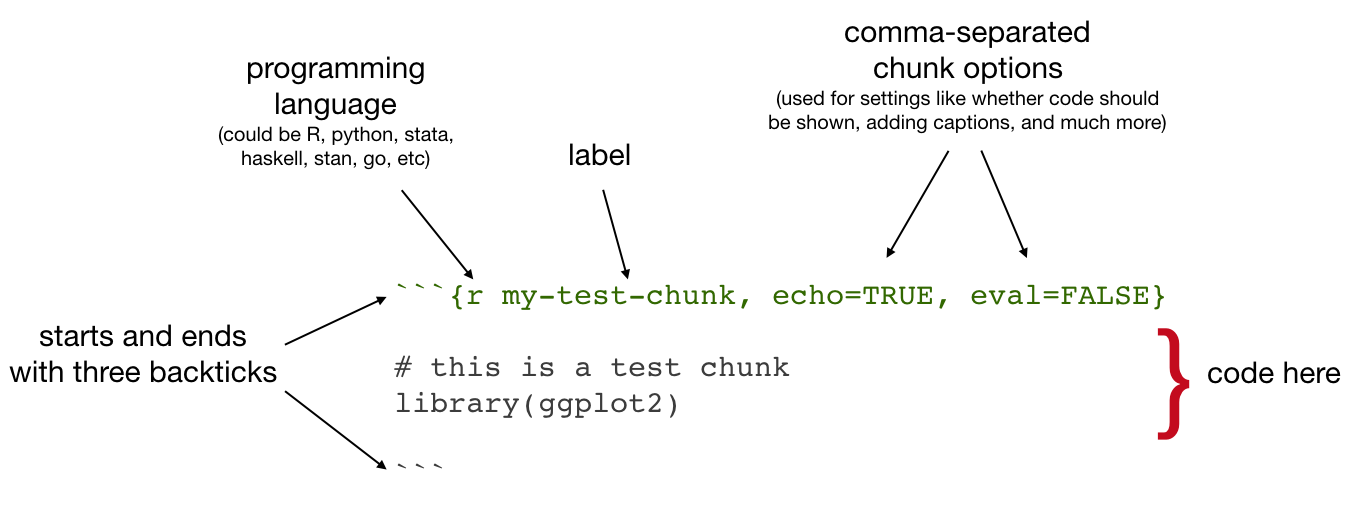
\includegraphics[width=1\linewidth]{figures/chunk-parts} \caption{Code chunk syntax}\label{fig:chunk-parts}
\end{figure}

Common chunk options include (see e.g.~\href{https://bookdown.org/yihui/rmarkdown/r-code.html}{bookdown.org}):

\begin{itemize}
\tightlist
\item
  \texttt{echo}: whether or not to display code in knitted output
\item
  \texttt{eval}: whether or to to run the code in the chunk when knitting
\item
  \texttt{include}: wheter to include anything from the from a code chunk in the output document
\item
  \texttt{fig.cap}: figure caption
\item
  \texttt{fig.scap}: short figure caption, which will be used in the `List of Figures' in the PDF front matter
\end{itemize}

\textbf{IMPORTANT}: Do \emph{not} use underscoores in your chunk labels - if you do, you are likely to get an error in PDF output saying something like ``! Package caption Error: \textbackslash caption outside float''.

\hypertarget{APD-study}{%
\chapter{APD study}\label{APD-study}}

\chaptermark{APD study}

\minitoc 

\hypertarget{introduction-4}{%
\section{Introduction}\label{introduction-4}}

\hypertarget{methods-4}{%
\section{Methods}\label{methods-4}}

\hypertarget{participants}{%
\subsection{Participants}\label{participants}}

Forty-four primary school children native British English speakers with normal hearing acuity participated in the study. Amongst them 20 belonged to the APD clinical group (5 females) with an average age of 11.04 \(\pm\)~1.42 years (range: 7.8 - 12.9 years). One APD child was excluded from the analysis due to raised thresholds (PTA\textgreater25~dB~HL). APD children were recruited in two ways. Children diagnosed with APD at Great Ormond Street Hospital (GOSH) and at the London Hearing and Balance Centre (LHBC), London, UK, and fulfilled the recruitment criteria were identified and contacted by a clinical team member. The parents/caregivers were provided with information about the study and means of contact to express interest in participation. Others were recruited by advertisements in social networks, where parents were requested to fill-out an interest form that included screening questions to ensure they fulfil the participation requirements. \colorbox[HTML]{CCCCFF}{To add percentage for clinics, diagnosed/LiD/susAPD and SPD pattern?} The remaining 23 (12 females) comprised of typically developing control children (TD) with no reported concerns or diagnosis of a language or other cognitive developmental disorders. The TD group average age was 9.47 \(\pm\)~1.58 years and ranged between 7 to 12.1 years (A detailed description of the groups is shown in Tab. ??).

Difference in variance for age between the two groups was tested using t-test with Welch degrees of freedom correction for uneven sample-size, showing a significant difference in age between the groups {[}t(40.95)=3.43, p=0.001{]}.

The project was approved by the UCL Research Ethics Committee (Project ID Number 0544/006) and the NHS Health Research Authority HRA (REC reference: 18/LO/0250). The testing commenced once an informed consent was given by both the parent/caregiver and the child.

\begin{itemize}
\tightlist
\item
  Background questionnaire
\item
  Otoscopic examination was carried out to ensure the eardrum is visible, healthy and intact.
\item
  Location of the testing
\item
  duration of the session
\end{itemize}

Participants from both TD and APD group completed the same battery of tests listed below

\hypertarget{auditory-evaluation}{%
\subsection{Auditory evaluation}\label{auditory-evaluation}}

\hypertarget{standard-audiometry}{%
\subsubsection{Standard audiometry}\label{standard-audiometry}}

\begin{figure}

{\centering \includegraphics[width=0.85\linewidth]{_main_files/figure-latex/PTA-1} 

}

\caption{APD participants pure-tone audiogram thresholds for standard frequencies plotted for the left and the right ear (black). The shaded grey area represents the TD group range of audiometric thresholds and the white line represents the mean at each frequency. The dashed line represents the threshold criteria of hearing level $\leq$ 25 dB HL.}\label{fig:PTA}
\end{figure}

A standard air conduction pure-tone audiometry was carried out at six octave frequency bands ranging between 0.25 to 8~kHz using ???? audiometer and ??? headphones. Normal hearing acuity was defined as thresholds \(\leq\) 25~dB~HL for the octave frequency bands between 0.25 to 4~kHz. Thresholds at 8~kHz were \(\leq\)~25~dB~HL for all the participants, excluding two participants with thresholds at 35 and 30~dB~HL in one ear, respectively. One participant from the clinical group (APD) was excluded from the analysis due to raised thresholds predominantly in the right ear (PTA\(_{Right}\) = 36.25~dB~HL; PTA\(_{Left}\) = 13.75~dB~HL). Otoscopy inspection of the child's ear canal revealed a large accumulation of cerumen whereby the right eardrum was not visible. The listeners' thresholds for the left and the right ear are plotted in Figure~\ref{fig:PTA}. The shaded grey area represents the TD group thresholds range and the white line represents their mean at each frequency. The black lines represents the individual thresholds in the APD group and the group mean is marked by the bold black line. The dashed line represents the maximal thresholds criteria of \(\leq\) 25~dB~HL for participation in the study. \colorbox[HTML]{CCCCFF}{Results belong here??}

\hypertarget{extended-high-frequency-audiometry-ehfa}{%
\subsubsection{Extended high-frequency audiometry (EHFA)}\label{extended-high-frequency-audiometry-ehfa}}

Extended high-frequency pure-tone audiometry was carried out at four \(\frac{1}{3}\) octave band frequencies 8, 11, 16, \& 20~kHz using a locally developed MATLAB based software which generated and collected the data. Measurements took place at SHaPS, UCL laboratory in an electromagnetically shielded sound proof booth which is typically used for EEG measurements. A Windows PC situated outside the booth was connected via USB to an RME ???? sound card (Audio AG, Haimhausen Germany) and an ER10X Extended-Bandwidth Acoustic Probe System (Etym\(\bar{o}\)tic Research, Elk Grove Village, IL) which was located in the testing booth. Once the ear probe was placed in the child's ear, an in-situ sound pressure level calibration was performed (chirp noise) using a MATLAB code provided by ????.

Speak with KZ about the measurements

\hypertarget{switching-task-st}{%
\subsubsection{Switching task (ST)}\label{switching-task-st}}

The switching task (ST) is a novel speech-on-speech listening task that involves perception of interrupted and periodically segmented speech that is switched between the two ears out-of-phase with an interrupted distractor. Since segments of the target and of the distractor are never presented in the same ear at the same time, it enables to eliminate peripheral (EM) masking, while maintaining high IM for speech distractors. The task assesses the ability to switch attention and integration of binaural information.

Refer to Chapter 2 and briefly describe the stimuli and difference in the methods.

As described in Chapter 2 Section ???, two test versions were used with varying in sentence structure and complexity: 1. ASL 2. CCRM

Masker Types..

\hypertarget{spatialised-speech-in-noise-lisns-uk}{%
\subsubsection{Spatialised speech-in-noise (LiSNS-UK)}\label{spatialised-speech-in-noise-lisns-uk}}

The Listening in Spatialised Noise Sentences UK (LiSNS-UK) assesses the ability to use binaural cues in speech-on-speech listening conditions. The test development, speech material normalisation, and norms standardisation followed \textcite{Cameron2007} development steps and are described in detail in Chapter ???. The test uses virtualisation techniques to create spatial distribution of sound sources in space for headphones presentation where target sentences \autocite[ASL;][]{MacLeod1990} are presented in two simultaneous speech distractors (unrelated children's stories spoken by the target talker). It comprises of two main listening conditions, differing in their availability of spatial cues. The target sentences are configured to always appear in front of the listener's head, at 0\(^{\circ}\) azimuth on the horizontal plane, with the two streams of speech distractors either co-located in space with the target (S0N0), resulting in relatively poor speech perception, or offset in space, with one distractor to either side of the target at \(\pm\)~90\(^{\circ}\), resulting in an improvement in speech perception of circa 13~dB \autocite{Cameron2011}, typically termed as spatial release from masking (SRM). This SRM advantage is calculated by taking the difference between performance in the co-located condition and the separated condition. The speech distractors were presented continuously throughout a run at a fixed 65?~dB~SPL output level and comprised of a combination of two out of three different passages children stories. A 1-up/1-down adaptive procedure was used, varying the level of the target talker relative to the distractors depending on listener's correct/incorrect response to measure the listeners' speech reception threshold (SRT), i.e., the signal-to-noise-ratio (SNR) yielding 50\% speech intelligibility. A 2~ms long 1~kHz pure-tone was presented 500~ms before the target sentence onset at 65?~dB~SPL (0 dB SNR) as a reference cue signalling the listener to attend the coming target sentence. The initial target output level was ??~dB~SPL with an initial step-size of 4~dB SNR. The step-size was reduced after every reversal, reaching a minimum step-size of 2~dB~SNR after three practice reversals. A stopping rule was introduced in case the maximal SNR was reached more than three times and the procedure was considered to be successfully completed in case test reversals were obtained. The SRT was then calculated by averaging test reversals SNRs (i.e., following three practice reversals). Each run consisted of 25 sentences taken from 8? phonemically-balanced test list which were constructed following the normalisation of the speech. In addition, a sentence-specific level correction was applied to the target signal (see Chapter ?? for more information). The order of the listening condition, test lists, target sentences and distractors combinations was fixed across all the participants and started with the collocated condition. Spatialisation was applied by convolving each stimuli with head-related transfer functions (HRTFs) at the corresponding azimuthal direction separately for the left and the right channel. The HRTFs were measured with a Knowles Electronics Manikin for Acoustic Research (KEMAR, REF) manikin with a small pinnae taken from the CIPIC HRTF database\footnote{The database is available online in: \url{https://www.ece.ucdavis.edu/cipic/spatial-sound/hrtf-data/}} {[}\textcite{Algazi2001}; see ``special'' HRTF data{]}. A post-equalisation step was applied in order to flatten the magnitude of the headphones frequency response. Headphone-to-ear Transfer Functions (HpTFs) measured with KEMAR manikin for HD-25 supraaural headphones were extracted from \textcite{Wierstorf2011} HRTF database. The final mixed stimulus was filtered with the inverse HpTFs separately for the left and the right channel before being combined together as a final step. Every participant was presented with two runs, one for each listening condition (collocated/separated). Testing started following a practice phase of two runs for each of the test conditions with five BKB sentences each \autocite{Bench1979}. Listeners were instructed to verbally repeat the target sentences to the experimenter who was situated alongside the participant in a sound treated chamber. The experimenter scored the response by selecting the correctly repeated keywords on the screen. Listeners were encouraged to guess if unsure while no feedback was given at any time. A loose keyword scoring method was used, whereby errors of case or declension were considered as correct responses. For example, a repetition of the keywords `\(<\)clown\emph{s}\(>\) \(<\)funny\(>\) \(<\)face\emph{s}\(>\)' to the stimulus `The \(<\)clown\(>\) had a \(<\)funny\(>\) \(<\)face\(>\)'.

\hypertarget{speech-in-noise-spin}{%
\subsubsection{Speech-in-noise (SPIN)}\label{speech-in-noise-spin}}

The speech-in-noise test was used as a more realistic listening situation that is widely used in the clinic as opposed to more complex listening tasks as listed above. The normalised ASL sentences were presented in a speech-shaped-noise (SSN) with spectrum matched to the ASL corpus. The SSN onset was 500~ms before the target sentence begin. The exact same adaptive procedure as for the LiSNS-UK was used with the same stop-rules. Each listener was presented with a single run of 25 sentences following a practice phase with seven BKB sentences. The same test list and sentences order was used across all the listeners.

\hypertarget{the-environmental-auditory-scene-analysis-task-envasa}{%
\subsubsection{The Environmental Auditory Scene Analysis task (ENVASA)}\label{the-environmental-auditory-scene-analysis-task-envasa}}

In analogy to the classic `cocktail-party' scenario, ENVASA is a non-linguistic paradigm \autocite{Leech2009} that measures detection of everyday environmental sounds presented in naturalistic auditory scenes and can be used to asses IM effects as well as sustained selective auditory attention skills. In the task, short environmental target sounds (e.g., a ``dog's bark'', ``door knock'' or ``bouncing ball'') were presented in a dichotic background scene (i.e., the target sound is presented only in one ear) consisting of either a single background scene,presented in both ears, or two background scenes, each presented in a different ear. The number of targets, the onset time and presentation ear varied across trials. Four target/background SNRs were employed split into two categories `low' (-6 and -3~dB) and `high' (0 and +3~dB) by varying the target level. Target/background contextual agreement was manipulated by embedding the target sound in a \emph{congruent} background scene that is in agreement with the listener's expectations (e.g., a cow's `moo' in a farmyard scene) or in an \emph{incongruent} background scene which violate these expectations (e.g., a cow's `moo' in a traffic scene).

Procedure:

The experiment was carried out using the original code and laptop as used and described by \textcite{Leech2009}. Sounds were presented via Sennheiser HD-25 headphones (REF) and the participants response was recorded using ???? gamepad. The output level was adjusted to a comfortable level before the test started. The participants were situated in front of the laptop placed on a desk and were instructed to hold the gamepad. Prior to the test begin the listeners were presented with a short child-friendly video covering the task's instructions and demonstrated two test trials. Following the instruction video, the examiner gave the child a short recap of the task's instructions and simulated with the child an exemplary trial to make sure the child is familiarised with the task. The task began with three practice trials with provided feedback, while no further feedback was given in the testing phase.

Every trial was made of two parts, starting with a target audio and visual familiarisation phase before the main target detection phase. Target identification was recorded by pressing one of the three buttons on the gamepad which corresponded to the location of the target objects on the screen. A response was counted as correct only if the participants pushed the corresponding button within 2~s time interval, 300~ms following the target onset. The outcome measure was calculated as the percentage of target sounds correctly identified within a condition (\%-correct).

In total there were 115 target sounds presented over 40 trials, where 46 target sounds were presented in a single background condition and another 46 in a dual-background condition. The 23 remaining target sounds served as foil items where they were played at 0~dB~SNR without a corresponding picture on the screen. The order of the foil items was quasi-randomised and were used to estimate the quality of the participants performance.



\begin{figure}

{\centering 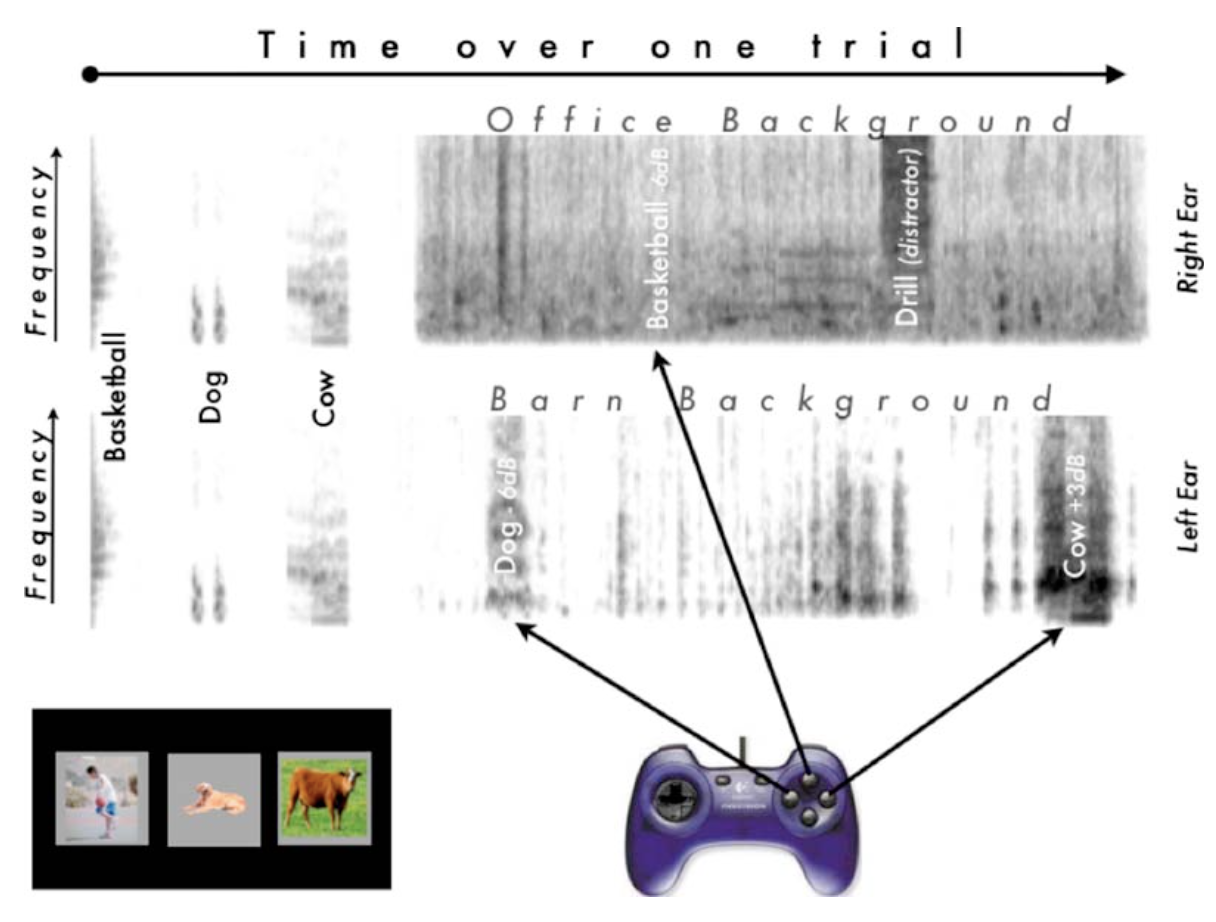
\includegraphics[width=0.65\linewidth]{figures/ENVASAparadigm} 

}

\caption{Schematic of the ENVASA experimental paradigm \autocite[taken from][]{Leech2009}}\label{fig:ENVASA}
\end{figure}

\hypertarget{celf-rs}{%
\subsubsection{CELF-RS}\label{celf-rs}}

The Recalling Sentences (RS) sub-test of the Clinical Evaluation of Language Fundamentals Fifth UK edition \autocite[CELF-5-UK][]{HWiig2017} was administered to assess the listeners expressive language ability and has been shown to be a good indicator of the listeners general language skills (REF). In the task the child is presented with pre-recorded sentences of increasing length and complexity and required to repeat sentences without any changes. Scoring were marked by hand by the examiner as instructed by the test manual. The sentences were spoken by a standard southern British English female and were recorded in a sound-treated recording booth at the SHaPS UCL laboratory, London. The sentences were presented using a MATLAB program via headphones using the same experimental equipment as listed above at a comfortable output level of 70~dB~HL. The task began with two practice sentences while the number of test items varied depending on the child's age performance. No repetitions or feedback was given during the testing and the test was discontinued in case the child failed to score any points for four consecutive items. Age-scaled score were calculated based on the test norms with a mean score of 10 and SD of 3. Scaled scores within \(\pm\)~1~SD from the norm mean (between 8 to 12) are classified as average scores, whereas performance beyond \(\pm\)~1~SD are classified as above/below the average score. Thus, the cut-off for abnormally poor performance is a scaled score \(\leq\)~7.

\hypertarget{questionnaires}{%
\subsection{Questionnaires}\label{questionnaires}}

\hypertarget{medical-neurological-and-pysiological-history}{%
\subsubsection*{Medical, Neurological, and Pysiological History}\label{medical-neurological-and-pysiological-history}}
\addcontentsline{toc}{subsubsection}{Medical, Neurological, and Pysiological History}

\hypertarget{the-evaluation-pf-childrens-listening-and-processing-skills-eclips}{%
\subsubsection*{The Evaluation pf Children's Listening and Processing Skills (ECLiPS)}\label{the-evaluation-pf-childrens-listening-and-processing-skills-eclips}}
\addcontentsline{toc}{subsubsection}{The Evaluation pf Children's Listening and Processing Skills (ECLiPS)}

The ECLiPS questionnaire \autocite{Barry2014} comprises of 38 items where the users are asked to express their agreement simple statements about the child's listening and other related skills or behaviours using a five-point Likert scale (from ``strongly agree'' to ``strongly disagree''). The ECLiPS was design to identify listening and communication difficulties in children aged 6 to 11 years. Nonetheless, the UK standardisation study (REF) found little to no age effect on scores in many of the scale items, suggesting the testing age could be extended below and beyond the population used for the development. Based on factor analysis the items are grouped into five subcategories: 1. Speech \& Auditory Processing (SAP), 2. Environmental \& Auditory Sensitivity (EAS), 3. Language, literacy \& laterality (L/L/L), 4. Memory \& Attention (M\&A), 5. Pragmatic \& Social skills (PSS). Age- and sex-scaled scores were computed using the test excel scorer.

A score below the 10\(^{th}\) percentile (corresponding to a scale score of circa 6) is generally considered clinically significant.

\hypertarget{the-childrens-communication-checklist-2nd-edition-ccc-2}{%
\subsubsection*{\texorpdfstring{The Children's Communication Checklist 2\(^{nd}\) edition (CCC-2)}{The Children's Communication Checklist 2\^{}\{nd\} edition (CCC-2)}}\label{the-childrens-communication-checklist-2nd-edition-ccc-2}}
\addcontentsline{toc}{subsubsection}{The Children's Communication Checklist 2\(^{nd}\) edition (CCC-2)}

Communication abilities were assessed using the Children's Communication Checklist second edition questionnaire \autocite[CCC-2;][]{D.V.M.2003} was completed by the child's parent/guardian. The CCC-2 was designed to screen communication problems in children aged 4 to 16 years and comprises of 70 checklist items each comprising of a behaviour statement like ``Mixes up words of similar meaning''. The respondents are asked to judge how often the behaviours occur using a four-point Likert rating scale: 0. \emph{less than once a week (or never)}, 1. \emph{at least once a week, but not every day}, 2. \emph{once or twice a day}, 3. \emph{several times (more than twice) a day (or always)}. The items are grouped into ten sub-scales of behaviours tapping into different skills (A. Speech, B. Syntax, C. Semantics, D. Coherence, E. Inappropriate initiation, F. Stereotyped language, G. Use of context, H. Non-verbal communication, I. Social relations, J. Interests). Taking the sum of scores for the sub-scales A to H are used to derive the General Communication Composite (GCC) which is used to identify clinically abnormal communication competence. A GCC score \textless{} 55 was found by \textcite{Norbury2005} to well separate between control and clinical groups, identifying children with scores at the bottom 10\%. Another composite (Social-Interaction Deviance Composite, SIDC) was taken by taking the difference in sum of scales E, H, I, and J from the sum of scales of A to D. Abnormal GCC (\textless~55) combined with a negative SIDC score has been shown to be indicative of an autistic spectrum disorder profile \autocite{D.V.M.2003}. The CCC-2 scaled and composite scores were computed using the test excel scorer. Data from one TD child out of forty four children was excluded from the analysis due to inconsistent reports flagged by the test scorer.

\hypertarget{results-3}{%
\section{Results}\label{results-3}}

\hypertarget{standard-audiometry-1}{%
\subsection{Standard audiometry}\label{standard-audiometry-1}}

\begin{figure}

{\centering \includegraphics[width=1\linewidth]{_main_files/figure-latex/stdAud-fig-1} 

}

\caption{Add caption here.}\label{fig:stdAud-fig}
\end{figure}

\begin{table}

\caption{\label{tab:stdAud-tab}Standard audiometry descriptive and test statistics for group differences tested using Wilcoxon rank-sum test for unpaired samples\textsuperscript{*}. PTA$_{Right}$ and PTA$_{Left}$ were calculated by taking the individual mean for thresholds at 0.5, 1, 2 and 4 kHz in the respective ear. PTA denotes the listeners grand-mean for PTAs in both ears and BE represents the listeners PTA at the better-ear.}
\centering
\resizebox{\linewidth}{!}{
\begin{tabular}[t]{lcccccc|>{}ccclc|>{}c>{}c>{}cc}
\toprule
\multicolumn{2}{c}{ } & \multicolumn{5}{c}{APD} & \multicolumn{5}{c}{TD} & \multicolumn{4}{c}{Wilcoxon rank-sum test} \\
\cmidrule(l{3pt}r{3pt}){3-7} \cmidrule(l{3pt}r{3pt}){8-12} \cmidrule(l{3pt}r{3pt}){13-16}
 & Ear & N & median & sd & min & max & N & median & sd & min & max & CI & p & effect size (r) & magnitude\\
\midrule
\addlinespace[0.3em]
\multicolumn{16}{l}{\textbf{octave frequency bands}}\\
\hspace{1em}250 & R & 20 & 10.00 & 3.73 & 0.00 & 15.00 & 23 & 5 & 3.95 & 0 & 15 & -0.00 - 5.00 & \em{0.35} & \em{0.14} & small\\
\hspace{1em}500 & R & 20 & 5.00 & 4.94 & 0.00 & 15.00 & 23 & 10 & 4.49 & -5 & 15 & -0.00 - 5.00 & \em{0.51} & \em{0.10} & small\\
\hspace{1em}1000 & R & 20 & 5.00 & 4.55 & -5.00 & 15.00 & 23 & 0 & 4.38 & -5 & 15 & -5.00 - 0.00 & \em{0.19} & \em{0.20} & small\\
\hspace{1em}2000 & R & 20 & 5.00 & 3.97 & 0.00 & 15.00 & 23 & 5 & 3.76 & 0 & 10 & 0.00 - 5.00 & \em{\textbf{0.03}} & \em{0.34} & moderate\\
\hspace{1em}4000 & R & 20 & 5.00 & 5.62 & -5.00 & 15.00 & 23 & 5 & 5.27 & -5 & 15 & -0.00 - 5.00 & \em{0.08} & \em{0.27} & small\\
\hspace{1em}8000 & R & 20 & 10.00 & 5.36 & 0.00 & 20.00 & 23 & 10 & 8.29 & -5 & 30 & 0.00 - 5.00 & \em{\textbf{0.00}} & \em{0.48} & moderate\\
\hspace{1em}250 & L & 20 & 5.00 & 4.99 & 0.00 & 20.00 & 23 & 5 & 5.05 & -5 & 15 & -0.00 - 5.00 & \em{0.29} & \em{0.16} & small\\
\hspace{1em}500 & L & 20 & 10.00 & 4.06 & 5.00 & 15.00 & 23 & 5 & 4.25 & -5 & 15 & -0.00 - 5.00 & \em{0.12} & \em{0.24} & small\\
\hspace{1em}1000 & L & 20 & 5.00 & 3.84 & 0.00 & 15.00 & 23 & 0 & 3.99 & -5 & 10 & -0.00 - 5.00 & \em{0.46} & \em{0.11} & small\\
\hspace{1em}2000 & L & 20 & 5.00 & 4.13 & 0.00 & 15.00 & 23 & 0 & 4.03 & -5 & 10 & -0.00 - 5.00 & \em{0.32} & \em{0.15} & small\\
\hspace{1em}4000 & L & 20 & 5.00 & 5.95 & -5.00 & 15.00 & 23 & 5 & 6.07 & -5 & 20 & -5.00 - 5.00 & \em{0.58} & \em{0.09} & small\\
\hspace{1em}8000 & L & 20 & 10.00 & 8.01 & 5.00 & 35.00 & 23 & 5 & 8.49 & -5 & 25 & -0.00 - 10.00 & \em{0.05} & \em{0.30} & small\\
\addlinespace[0.3em]
\multicolumn{16}{l}{\textbf{PTAs and better-ear}}\\
\hspace{1em}PTA$_{Right}$ & R & 20 & 4.38 & 3.78 & -1.25 & 12.50 & 20 & 5 & 5.62 & -5 & 15 & -1.25 - 3.75 & \em{0.56} & \em{0.09} & small\\
\hspace{1em}PTA$_{Left}$ & L & 20 & 5.00 & 3.04 & 0.00 & 11.25 & 20 & 10 & 5.36 & 0 & 20 & 1.25 - 5.00 & \em{\textbf{0.01}} & \em{0.42} & moderate\\
\hspace{1em}PTA &  & 20 & 5.31 & 2.92 & 0.62 & 10.62 & 20 & 5 & 4.99 & 0 & 20 & -0.00 - 3.75 & \em{0.08} & \em{0.27} & small\\
\hspace{1em}BE &  & 20 & 3.75 & 3.17 & -1.25 & 8.75 & 20 & 10 & 4.06 & 5 & 15 & -1.25 - 3.75 & \em{0.23} & \em{0.18} & small\\
\bottomrule
\multicolumn{16}{l}{\textsuperscript{*} significant p-values (p < 0.05) are shown in bold.}\\
\end{tabular}}
\end{table}

Boxplots of listeners thresholds measured with a standard audiometer at the six octave frequency bands (0.25 to 8~kHz) and their corresponding PTAs are shown in Figure~\ref{fig:stdAud-fig}~A-B. The listeners PTAs were calculated separately for the right and left ear (PTA\(_{Right}\), PTA\(_{Left}\)) by taking the mean of thresholds at the frequency bands 0.5, 1, 2 and 4~kHz which are known to be important for speech perception (REF WHO). PTA denotes the listeners grand-mean for PTAs in both ears, form a single measure for the listeners hearing ability, and BE represents the listeners PTA at the better-ear. Descriptive statistics is given in Table~\ref{tab:stdAud-tab}, split by groups.

\colorbox[HTML]{CCCCFF}{Do the groups differ in their hearing abilities?}\\
- To report Wilcoxon or LMEM test? - Wilcoxon test and LMEM found a significant difference between the groups for thresholds in the left ear. Nonetheless, the differences are rather small and clinically negligible, and there is no reason to assume this difference occurred by random.

\hypertarget{extended-high-frequency-audiometry-ehfa-1}{%
\subsection{Extended high-frequency audiometry (EHFA)}\label{extended-high-frequency-audiometry-ehfa-1}}

\begin{figure}

{\centering \includegraphics[width=1\linewidth]{_main_files/figure-latex/EHFAud-fig-1} 

}

\caption{Add caption here.}\label{fig:EHFAud-fig}
\end{figure}

\begin{table}

\caption{\label{tab:EHF-tab}Extended high frequency hearing screening descriptive statistics and group difference analysis by frequency and ear or PTA.}
\centering
\resizebox{\linewidth}{!}{
\begin{tabular}[t]{lcccccc|>{}ccclc|>{}c>{}c>{}cc}
\toprule
\multicolumn{2}{c}{ } & \multicolumn{5}{c}{APD} & \multicolumn{5}{c}{TD} & \multicolumn{4}{c}{Wilcoxon rank-sum test} \\
\cmidrule(l{3pt}r{3pt}){3-7} \cmidrule(l{3pt}r{3pt}){8-12} \cmidrule(l{3pt}r{3pt}){13-16}
 & Ear & N & median & sd & min & max & N & median & sd & min & max & CI & p & effect size (r) & magnitude\\
\midrule
\addlinespace[0.3em]
\multicolumn{16}{l}{\textbf{octave frequency bands}}\\
\hspace{1em}11000 & R & 19 & 10.00 & 11.19 & 0.00 & 45.0 & 22 & 10.00 & 13.24 & 0 & 45.0 & -5.00 - 10.00 & \em{0.47} & \em{0.11} & small\\
\hspace{1em}16000 & R & 18 & 2.50 & 10.04 & 0.00 & 30.0 & 21 & 0.00 & 10.51 & 0 & 35.0 & -0.00 - 10.00 & \em{0.14} & \em{0.23} & small\\
\hspace{1em}11000 & L & 19 & 10.00 & 11.65 & 5.00 & 45.0 & 22 & 10.00 & 10.71 & 0 & 40.0 & -0.00 - 5.00 & \em{0.57} & \em{0.09} & small\\
\hspace{1em}16000 & L & 19 & 5.00 & 13.80 & 0.00 & 40.0 & 21 & 0.00 & 8.11 & 0 & 25.0 & -0.00 - 10.00 & \em{0.21} & \em{0.20} & small\\
\addlinespace[0.3em]
\multicolumn{16}{l}{\textbf{PTAs and better-ear}}\\
\hspace{1em}PTA$_{Right}$ & R & 19 & 7.50 & 9.74 & 0.00 & 32.5 & 22 & 5.00 & 12.42 & 0 & 40.0 & -2.50 - 5.00 & \em{0.48} & \em{0.11} & small\\
\hspace{1em}PTA$_{Left}$ & L & 19 & 7.50 & 12.28 & 2.50 & 42.5 & 22 & 7.50 & 9.62 & 0 & 35.0 & -2.50 - 7.50 & \em{0.27} & \em{0.18} & small\\
\hspace{1em}PTA &  & 19 & 8.75 & 10.18 & 1.25 & 37.5 & 22 & 6.25 & 10.57 & 0 & 37.5 & -2.50 - 6.25 & \em{0.29} & \em{0.17} & small\\
\hspace{1em}BE &  & 19 & 7.50 & 8.95 & 0.00 & 32.5 & 22 & 3.75 & 10.09 & 0 & 35.0 & -2.50 - 5.00 & \em{0.24} & \em{0.18} & small\\
\bottomrule
\end{tabular}}
\end{table}

The listeners' thresholds measured with the ER10X at the EHFs 11 and 16~kHz are plotted in Figure \ref{fig:EHF} for the left and the right ear. The shaded grey area represents the TD group thresholds range and the white line represents their mean at each frequency. The black lines represents the individual thresholds in the APD group and the group mean is marked by the bold black line. A comparison of the group means indicates that the differences in thresholds are small. Again, boxplots of the listeners thresholds by frequency and ear as well as PTAs are shown in Figure~\ref{fig:EHFAud-fig} A-B. Descriptive statistics and Wilcoxon rank-sum test outcomes for group comparison (unpaired samples) is given in Table~\ref{tab:EHF-tab}, split by groups.

\colorbox[HTML]{CCCCFF}{Difference between groups} Difference in thresholds between the groups across frequencies (11 \& 16~kHz) and ears (left/right) as well as for the calculated PTA and BE measures were tested using a Wilcoxon rank-sum test for unpaired samples (`rstatix::wilcox\_test' with bonferroni adjustment; REF). No significant difference was found between the groups for all thresholds (all p\textgreater.05; see Table~\ref{tab:EHF-tab}). A LMEM model with \textbf{frequency} and \textbf{ear} as fixed factors showed similar results and thus was not reported here.

\begin{figure}

{\centering \includegraphics[width=0.85\linewidth]{_main_files/figure-latex/EHF-1} 

}

\caption{APD participants pure-tone thresholds for extended high-frequencies plotted for the left and the right ear (black). The shaded grey area represents the TD group range of audiometric thresholds and the white line represents the mean at each frequency.}\label{fig:EHF}
\end{figure}

\hypertarget{switching-task-st-1}{%
\subsection{Switching task (ST)}\label{switching-task-st-1}}

\hypertarget{data-analysis}{%
\subsubsection*{Data Analysis}\label{data-analysis}}
\addcontentsline{toc}{subsubsection}{Data Analysis}

\colorbox[HTML]{CCCCFF}{\emph{Outliers \& missing data}}

As a first step, the listeners adaptive track and psychometric functions (PF) were manually inspected for abnormalities. The proportion of correct keywords within the final test trials (LevsPC) was calculated as a measure describing the success of the adaptive procedure. Since the adaptive procedure was set to yield 50\%-correct, a successful procedure is expected to be within the 50\% range. A binomial statistical test was applied to identify observations that significantly differ from 50\%. Observations with LevsPC~\(\leq\)~35\% were flagged as possible outliers and were further inspected (see Figure ??). Interestingly, the majority of the flagged cases belonged to the CCRM test condition where targets were presented with a competing CCRM-type sentences (CCRM\_F). Three observations out of 215 (5 conditions x 43 listeners) were flagged for data measured with the ASL corpus, and 29 observations out of 258 (6 conditions x 43 listeners) were flagged for data measured with the CCRM corpus. As expected, most of the identified cases were for observations measured with the more demanding conditions with speech distractors (see Figure ??). In five cases (2 ASL; 3 CCRM) we were able to confidently determine that the listener's true score was near to ceiling, and thus these observations were set to the maximum DC (0.97). In other cases it was not possible to confidently determine the true SRdT, either because the maximum number or trials were presented before a minimum number of test reversals were obtained (CCRM~=~1; ASL~=~2), or due to aberrant adaptive tracks (CCRM~=~5). Since all these cases belonged to more challenging test conditions with speech distractors, it is very likely that the children's true score is at celling. Thus, to account that, rather than removing these observations, which will consequently reduce the statistical power, they were set to a DC of 1, which is above the task's upper DC limit of 0.97.

\colorbox[HTML]{CCCCFF}{\emph{Regression lines + z-scores}}

Age-independent scores were estimated using a linear regression model. The model was fitted condition-wise separately for each test version (ASL/CCRM) and was based on the control group data only with \%-correct as the dependent variable and age as a predictor. A two-steps model comparison was performed to test the assumption that performance displays a monotonic linear relationship with age versus a non-monotonic (segmented) linear relationship. Extreme outliers were initially trimmed from the TD group to reduce noise in the data and to improve the models fit. In the first step, both models were computed and the best model was selected based on F-statistic model comparison using analysis of variance \textbf{anova()} test. Standard residuals were next calculated for each TD listener, based on the selected model prediction. The standardised residuals are age-independent and are comparable to z-scores for data with normal distribution, with a mean and SD of approximately 0 and 1, respectively. Since the main goal of the study was to find a measure that is able to well separate between the APD group and the typically developed control group, individual differences and group differences were explored using a deviance analysis procedure proposed by \textcite{Ramus2003}. Abnormal scores were defined by a two-tailed deviance cut-off of \(\pm\)~1.96~SD from the TD group mean. Thus, circa 95\% of the normal population residuals are expected to be within the deviance range of \(\pm\)~1.96. Occasional occurrence of abnormal scores in the normal population is not unusual in behavioural measures. Therefore, since the prediction of the residuals is based on the control data, such outliers may skew the TD group true mean or SD and thus may introduce an error in the model prediction. Therefore, in the second step, additional TD outliers (with standardised residuals below/above TD mean \(\pm\)~1.96) were trimmed from the data and the two models were refitted and compared again. Finally, the model with the best fit was selected and was used to calculate the standardised residuals for all the listeners, including the trimmed TD observations and the APD group.

\colorbox[HTML]{CCCCFF}{\emph{Age effect}}

The effect of age was analysed using the trimmed TD group data only. This is because the control group is more heterogeneous, and thus we expect performance in the TD group to be less variable than in the APD group. A repeated measures factorial design LMEM model was used with Condition, Material (ASL/CCRM) and Age as fixed factors, SRdT as dependent variable and a random intercept for subjects. A model without three-way interaction between the main effects was found to give the best fit. Inspection of the data revealed that the assumption of normal distribution (Shapiro Wilk test) was met, whereas the assumption of homogeneity of variance (Levene's test) was marginal (\emph{p=0.04}).

\colorbox[HTML]{CCCCFF}{\emph{Group, material and condition differences for z-scores}}\\
A 2x2x5 factorial design model with repeated measures was used to determine the effects of Group, Condition and Material as well as their interaction on the age-independent calculated z-scores. Residual analysis of a three-way ANOVA test was performed to determine if the model fulfils parametric methods assumptions. Shapiro-Wilk normality test (REF) rejected the assumption that the residuals were normally distributed, while the assumption of homoscedasticity was met (p\textgreater~0.05; Levene's test, REF).

Due to the violation of normality and possible sphericity violations a nonparametric method was performed using nparLD package (REF) which is a robust rank-based method for analysis of skewed data or with outliers or from a small sample size (REF J. Feys, 2016 New parametric TankTest). The analysis was based on a f2-ld-f1 design ANOVA-type statistic (ATS) test, whereby f2 refers to an experimental design with two between-subjects factors (Group \& Material) and f1 refers to a single within-subjects factor (Condition).

other tests were considered and delivered the same results!!

\hypertarget{srdts-by-age}{%
\subsubsection*{SRdTs by age}\label{srdts-by-age}}
\addcontentsline{toc}{subsubsection}{SRdTs by age}

Since the age of the TD/APD children that participated in the present study spanned between circa 7 to 13 years, a developmental age effect was expected, where performance was expected to improve with an increasing age. To inspect this effect across the different test conditions and speech material (ASL/CCRM), scatterplots and linear regression lines for the listeners SRdTs as a function of age are shown in Figure~\ref{fig:ST-Age}~A-B. The effect of age was tested against the TD group only since the variability in scores in the TD group is expected to be relatively smaller than in the clinical APD group. Therefore, any interpretation based on the APD regression lines should be carried out cautiously. The TD regression lines were determined based on model comparison and outliers trimming procedure to improve the model's fit (see section ??). Regular regression lines were found to be the most parsimonious in describing the relationship between the TD children performance and their age. This was the case in all test conditions but the MDR\_F distractor in the ASL material, where a segmented line was found to give the best fit. MDR\_F segmented line indicated that DC improved with age by circa 0.1 per year until reaching a plateau at the age of 9.5 years.

\begin{figure}[h]

{\centering \includegraphics[width=1\linewidth]{_main_files/figure-latex/ST-Age-1} 

}

\caption{Scatterplot and linear regression lines for the listeners SRdTs measured with the switching task with the ASL (A) and CCRM speech material (B) as a function of age. Corresponding regression coefficients and statistics is provided for TD group only. Red indicates data from the APD group and cyan indicates data from the TD control group. Data for normal hearing adults taken from Chapter 2 is shown in the boxplots as a reference.}\label{fig:ST-Age}
\end{figure}

Overall, Figure \ref{fig:ST-Age}~A-B showed a similar trend in performance in the two speech materials, where children in both groups showed larger decrement in performance for speech distractors (smaller SRdT \(\rightarrow\) better performance). The regression lines indicates that the improvement in performance by age was more prominent for speech distractors, with relatively steeper slopes (almost twice as steep) than for the non-speech distractor (AMSSN) or for conditions without a distractor. Furthermore, as expected, CCRM sentences were more intelligible, with performance shifted towards lower DC range (i.e., more difficult) relative to performance for the ASL speech material. This is due to the more simple speech material and the restricted alternative responses of the CCRM matrix-based sentences.

A closer look at the linear lines shows several interesting trends. The non-speech AMSSN distractor showed to have little-to-no effect on performance, at least in the TD group, where performance was fairly similar to performance in the Quiet conditions. When comparing the regression lines, there appears to be a relatively larger separation between the groups for data measured with the CCRM speech material, especially for AMSSN, but also for the speech distractors. However, it is possible that the APD regression lines do not reflect the true population due to the large spread in performance and the small sample size and thus any interpretation should be taken with a pinch of salt. Another interesting observation is that the children showed little-to-no \emph{masking-release} for speech spoken in an unfamiliar language (MDR\_F) when compared with a distractor spoken in English (ENG\_F). This is in agreement with findings in the adults study in Chapter~\ref{Chpt2}. Lastly, it is apparent from the figure that performance for CCRM\_F distractor was near-to-ceiling for some children, mostly among the APD group.

An exploratory comparison between between the children's data measured in the present study with data measured across young NH adults collected in Chapter~\ref{Chpt2} further highlight the strong developmental trend, with SRdTs still not entirely ``adult-like'' even at the age of 13 years, especially for speech distractos (see boxplots in Figure~\ref{fig:ST-Age}~A-B). The children in both groups seems to be markedly susceptible to competing CCRM sentences or familiar/unfamiliar speech presented with ASL sentences, with performance at the age of 12 years still largely differing from those obtained by the adults. On the other hand, by the age of 12 years, the TD children reached near to ``adult-like'' performance when CCRM target sentences were presented with with ENG\_F speech distractor or when ASL sentences were presented with AMSSN distractor.

Next, age effect was evaluated using LMEM (lmer, REF), with Condition, Material (ASL/CCRM) and Age as fixed factors, SRdT as dependent variable and a random intercept for subjects (reference levels: Condition = Quiet-NoAlt; Material = ASL). A model without two-way interaction between Condition, Material and Age was found to give the best fit (see Table~\ref{tab:ST-AgeLMEM}). Model comparison procedure was performed on the model with the best fit, comparing it to a reduced model where each of the fixed terms were singly term was removed, starting with the interaction terms. The model comparison revealed a highly significant two-way interaction between Condition~x~Age (p\textless0.001) as well as a marginal two-way interaction between Condition~x~Material and Material~x~Age (p=0.052). These results further supports the trends seen in the scatterplots.

\textcolor{red}{The significant Material x Age interaction indicates that the developmental trend is different between the two speech materials, with larger age effect (i.e., steeper slopes) for the ASL than for the CCRM sentences(?????). [the LMEM summary gives an estimate for materialCCRM:Age of 0.014 (ASL is the reference level). Does that mean that the ASL sentences mean improvement per 1 year was 0.014 larger than for the CCRM material? I'm not too sure how to interpret this..]} Furthermore, the significant Condition~x~Material interaction implies that performance in the different test conditions differed between the two speech materials. A post-hoc t-test comparison based on the fitted model (lsmeans(), REF; see Table~\ref{tab:ST-AgeLMEMpost}), revealed a highly significant difference in performance between the speech materials (reference level = ASL) across all five test conditions (all p's \textless~0.001). The estimated mean difference between the contrast pairs ranged between +0.18 to +0.27, hence, the CCRM speech material was significantly more intelligible than the ASL material, across all test conditions.

Lastly, as observed in Figure~\ref{fig:ST-Age}~A-B, the highly significant Condition~x~Age interaction supports the observation that the magnitude of the age effect was different across the test conditions. These findings raises the following questions -- do all the conditions show a significant age effect? Moreover, since the effect of age is not the same across the test conditions, which conditions showed the largest age effect? One possible way to tackle these questions is to compare the separate regression models using F-statistics. Nonetheless, due to the small sample-size and the large number of paired comparisons, the test lacks a statistical power, thus the results may not reflect the true effect (better term?). The TD group regression model's R\(^{2}\) and p-values are given in the bottom part of Figure A and B. The ASL model's p-value showed a highly significant age effect for ENG\_F, MDR\_F and Quiet-NoAlt condition and a marginal effect for AMSSN (p=0.048), whereas no significant age effect was found for Quiet-Alt (p=0.168). As for the CCRM material, there was a highly significant age effect for ENG\_F and a marginal effect for the Quiet-Alt condition (p=0.058) and for CCRM\_F condition (p=0.05) which is not included in the LMEM model, whilst no significant age effect was found for Quiet-NoAlt, AMSSN and MDR\_F conditions. Furthermore, age was found to be a better predictor (i.e., accounting for larger variance in SRdT) for conditions with speech distractors, with R\(^{2}\) ranging between 32\% to 72\% for the ASL material and about 12\% to 29\% for the CCRM material. A comparison between the regression lines slopes fitted for the different test conditions for the CCRM (x-axis) and ASL speech material (y-axis) is depicted in Figure~\ref{fig:ST-AgeSlopes}. A possible pattern emerges from the figure, namely, while the slopes for the quiet and non-speech conditions are fairly similar across the two speech material (indicated by their proximity to the diagonal line), differences are relatively larger for speech distractors, in particularly for MDR\_F where the slope for the ASL material (-0.13) is about six times steeper than the slope for the CCRM material (-0.02).

\begin{table}

\caption{\label{tab:ST-AgeLMEM}Mixed effects model for SRdTs measured with the switching task with condition, speech material and age as fixed factors and a random intercept for subjects. Note: only data measured with the control group following outliers trimming was included (trimmed TD). Reference levels: Condition = Quiet-NoAlt, Group = APD, Material = ASL).}
\centering
\begin{tabular}[t]{>{\raggedright\arraybackslash}p{8cm}cc>{}c}
\toprule
\multicolumn{4}{l}{SRdT \textasciitilde{} Condition + Material + Age} \\
\multicolumn{4}{c}{+ CondCode:material + CondCode:Age + material:Age + (1 | Subjects)} \\
\cmidrule(l{3pt}r{3pt}){1-4}
Main effects & Df & $\chi^{2}$ & p\\
\midrule
Condition:Material & 4 & 9.385 & \em{\textbf{0.052}}\\
Condition:Age & 4 & 14.919 & \em{\textbf{0.005}}\\
Material:Age & 1 & 3.786 & \em{\textbf{0.052}}\\
\bottomrule
\multicolumn{4}{l}{\textsuperscript{*} significant p-values (p < 0.05) are shown in bold.}\\
\end{tabular}
\end{table}



\begin{table}

\caption{\label{tab:ST-AgeLMEMpost}Post-hoc t-test paired comparison for Condition x Material two-way interaction. The test was performed on the fitted LMEM model and included adjusted least-squared-mean for the random intercept (subjects) using lsmeans package (REF).}
\centering
\resizebox{\linewidth}{!}{
\begin{tabular}[t]{lcccc>{}cc}
\toprule
Contrasts & Estimate & SE & Df & t-value & p-value & 95\%-CI\\
\midrule
(Quiet-NoAlt ASL) - (Quiet-NoAlt CCRM) & 0.19 & 0.03 & 216.45 & 7.62 & \em{\textbf{< 0.001}} & 0.14 - 0.24\\
(Quiet-Alt ASL) - (Quiet-Alt CCRM) & 0.20 & 0.03 & 216.21 & 8.01 & \em{\textbf{< 0.001}} & 0.15 - 0.25\\
(AMSSN-Alt ASL) - (AMSSN-Alt CCRM) & 0.18 & 0.03 & 216.25 & 7.37 & \em{\textbf{< 0.001}} & 0.14 - 0.23\\
(MDR\_F-Alt ASL) - (MDR\_F-Alt CCRM) & 0.24 & 0.03 & 216.21 & 9.66 & \em{\textbf{< 0.001}} & 0.19 - 0.29\\
(ENG\_F-Alt ASL) - (ENG\_F-Alt CCRM) & 0.27 & 0.03 & 216.21 & 10.90 & \em{\textbf{< 0.001}} & 0.22 - 0.32\\
\bottomrule
\multicolumn{7}{l}{\textsuperscript{*} significant p-values (p < 0.05) are shown in bold.}\\
\end{tabular}}
\end{table}

\begin{figure}

{\centering \includegraphics[width=0.6\linewidth]{_main_files/figure-latex/ST-AgeSlopes-1} 

}

\caption{A comarison beteween the regression lines slopes fitted for the CCRM (x-axis) and ASL speech material (y-axis) in the switching task. The different test conditions are represented by the different symbols given in the legend. The diagonal line represents an optimal agreement between the speech materials. Observations falling below the line indicate steeper slope for the ASL material than compared with the CCRM material.}\label{fig:ST-AgeSlopes}
\end{figure}

\hypertarget{age-independent-z-scores}{%
\subsubsection*{Age-independent z-scores}\label{age-independent-z-scores}}
\addcontentsline{toc}{subsubsection}{Age-independent z-scores}

\colorbox[HTML]{CCCCFF}{\emph{Boxplots \& abnormal scores by conditions}}

Age-independent (standardised residuals) z-scores were calculated based on the TD group data using a multiple-case study approach (\textcite{Ramus2003}; see section ??? for more details). Descriptive statistics for the listeners age-independent z-scores is giving in Table~\ref{tab:ST-Tab}. Additional boxplots are shown in Figure~\ref{fig:ST-z}~A-B, for the ASL and CCRM speech material respectively. Scores were calculated separately for each test condition, with better performance indicated by smaller z-score. The grey area marks the two-tailed 1.96 deviance cut-off for abnormal score from the control group mean (z~\(\approx\)~0), where only about 5\% of the normal population is expected to score below/above it. Overall, APD children performance in both test versions was noticeably poorer, with higher median z-scores than compared with the TD children. The next paragraphs will cover the examination and analysis of the individuals and group differences separately for each test version.

\begin{figure}

{\centering \includegraphics[width=1\linewidth]{_main_files/figure-latex/ST-z-1} 

}

\caption{Boxplots of the listeners age-independent standardised residuals for data measured with the ASL (A) and the CCRM speech material (B). Residuals were calculated seperately for each condition and are based on a model predicton for TD group only. The grey area represents the deviance cut-off for abnormal score (SD $\pm$ 1.96 below/above the TD mean), where about 95\% of the normal population is e expected to lay within. The dashed line represents the theorethical TD group mean (z = 0).}\label{fig:ST-z}
\end{figure}

\begin{table}

\caption{\label{tab:ST-tab}Switching task descriptives for standardised residuals (z-scores) calculated for data measured with the ASL and CCRM speech material.}
\centering
\resizebox{\linewidth}{!}{
\begin{tabular}[t]{lccccc|>{}ccccc}
\toprule
\multicolumn{1}{c}{ } & \multicolumn{5}{c}{APD} & \multicolumn{5}{c}{TD} \\
\cmidrule(l{3pt}r{3pt}){2-6} \cmidrule(l{3pt}r{3pt}){7-11}
 & N & median & sd & min & max & N & median & sd & min & max\\
\midrule
\addlinespace[0.3em]
\multicolumn{11}{l}{\textbf{ASL}}\\
\hspace{1em}Quiet-NoAlt & 20 & 1.81 & 1.39 & -0.76 & 3.74 & 23 & 0.00 & 1.96 & -1.69 & 6.05\\
\hspace{1em}Quiet-Alt & 20 & 0.29 & 0.87 & -0.79 & 2.12 & 23 & -0.13 & 1.46 & -1.72 & 5.27\\
\hspace{1em}AMSSN-Alt & 20 & 1.79 & 1.45 & -0.82 & 4.50 & 23 & 0.10 & 2.35 & -2.18 & 9.04\\
\hspace{1em}MDR\_F-Alt & 20 & 0.99 & 1.75 & -1.31 & 5.37 & 23 & -0.13 & 1.11 & -1.44 & 2.91\\
\hspace{1em}ENG\_F-Alt & 20 & 0.90 & 1.53 & -2.96 & 3.09 & 23 & 0.12 & 1.55 & -4.44 & 1.75\\
\addlinespace[0.3em]
\multicolumn{11}{l}{\textbf{CCRM}}\\
\hspace{1em}Quiet-NoAlt & 20 & 0.36 & 1.75 & -1.73 & 5.70 & 23 & 0.38 & 1.57 & -1.92 & 5.72\\
\hspace{1em}Quiet-Alt & 20 & 0.47 & 1.23 & -1.66 & 3.58 & 23 & -0.08 & 1.19 & -1.68 & 3.44\\
\hspace{1em}AMSSN-Alt & 20 & 1.62 & 2.03 & -1.39 & 7.95 & 23 & -0.28 & 1.09 & -1.38 & 2.50\\
\hspace{1em}MDR\_F-Alt & 20 & 0.86 & 1.40 & -1.12 & 4.06 & 23 & 0.28 & 1.11 & -1.87 & 2.77\\
\hspace{1em}ENG\_F-Alt & 20 & 1.05 & 1.22 & -0.80 & 3.25 & 23 & 0.26 & 1.14 & -1.80 & 2.99\\
\hspace{1em}CCRM\_F-Alt & 20 & 1.11 & 0.89 & -1.59 & 2.24 & 23 & 0.24 & 0.98 & -1.76 & 1.47\\
\bottomrule
\end{tabular}}
\end{table}

\hypertarget{asl-corpus}{%
\paragraph*{ASL corpus}\label{asl-corpus}}
\addcontentsline{toc}{paragraph}{ASL corpus}

A comparison of the groups means reveals that the APD children were more susceptible to the non-switched condition (Quiet-NoAlt), where the target sentences were presented in quiet, and the switched condition where the target sentences were presented with a non-speech distractor (AMSSN), which yielded the largest separation between the groups, with APD median score of 1.81 and 1.79, respectively, laying just within the norms upper limit. Performance of the APD children was also noticeably poorer for conditions with speech distractors (MDR\_F and ENG\_F), with median z-score of circa 1, whereas performance for Quiet-Alt condition was fairly similar between the groups.

A comparison between the proportion of abnormal scores amongst the APD children in the different conditions revealed that AMSSN, Quiet-NoAlt and MDR\_F gave the highest proportion of abnormal scores\footnote{Focusing on future clinical viability of the task, we were only interested in identifying children with clinically poor performance. Thus, abnormal score was defined as a one-tailed deviance cut-off of z-score \textgreater{} 1.96, within which circa 97.5\% of the normal population is expected to lay.}.
Surprisingly, AMSSN distractor yielded the highest proportion of abnormal scores, with half of the APD children exhibiting abnormal score (20/10, 50\%). Followed by Quiet-NoAlt condition, where paradoxically and against our expectation 45\% of the APD group (9/20) obtained an abnormal score, whereas only 10\% (2/20) obtained an abnormal score in the Quiet-Alt condition. Interestingly, the APD children did not benefit from a release of masking for a speech distractor spoken in an unfamiliar language (MDR\_F) as opposed to a familiar speech spoken in English (ENG\_F), with median scores very similar in both conditions. This sits well with our previous findings with adults where adults showed no benefit for MDR\_F speech masker (see chapter ???). Another interesting observation was that double the amount of APD children exhibited abnormal score (8/20~=~40\%), making it the third largest proportion of abnormal scores, while only 20\% (4/20) of the children were abnormal for the ENG\_F condition. Lastly, The proportion of abnormal scores amongst the TD group ranged between 0\% to 13\% with a mean of 7.8\%, which corroborate fairly well with the theoretical probability of 2.5\% (one-tailed).

\hypertarget{ccrm-corpus}{%
\paragraph*{CCRM corpus}\label{ccrm-corpus}}
\addcontentsline{toc}{paragraph}{CCRM corpus}

Figure \ref{fig:ST-z}~B reveals a similar trend for the CCRM sentences, however with a more modest differences between the two groups. AMSSN yielded the largest separation between the groups, where 40\% (8/20) of the APD children obtained an abnormal score and with a median score of 1.62, which is relatively close to the +1.96 upper deviance cut-off. In comparison, only 4.3\% of the TD children (1/23) had abnormal performance for AMSSN condition. Again, the APD group median z-score for the speech distractors conditions was approximately 1 (range: 0.86-1.11), however the proportion of abnormal APD children was noticeably smaller than for the non-speech distractor, with 25\% (5/20) for MDR\_F, 20\% (4/20) for ENG\_F, and only 10\% (2/20) for CCRM\_F distractor. Lastly, in contrast to the ASL material, performance for the CCRM sentences presented in quiet were relatively better without switching (NoAlt) than with switching (Alt). Nonetheless, the spread in performance for the non-switched condition was larger, which suggests that some APD children were more negatively affected by the condition than others. The percentage of abnormal scores in the TD group were relatively low ranging between 0 to 8.7\% (2/23, Quiet-NoAlt) with an average of 4.3\% abnormal scroes across the different conditions.

\colorbox[HTML]{CCCCFF}{\emph{nparLD() full 2x2x5 model}}

A three-way 2~x~2~x~5 factorial design with repeated measures was used to test the main effects of Group, Condition, and Material as well as their interaction on performance in the task (with z-scores as dependent variable). Note that the CCRM test condition with CCRM-type sentences as distractor (CCRM\_F) was not included in the model since there was no comparable condition in the ASL speech material. Inspection of the standardised residuals z-scores revealed that the assumption of normal distribution (Shapiro Wilk test) was rejected for data measured with both speech material. Furthermore, homogeneity of the variance in the APD group was rejected for the ASL corpus (Levene's test; \emph{F(4,95)~=~2.71}, \emph{p~\textless~0.05}). Thus, due to the small sample size and the incomplete fulfilment of parametric statistical methods assumptions, a non-parametric approach was adopted. This was tested with an rank-based ANOVA-type statistic test (ATS) using the \emph{nparLD()} function (nparLD package, REF), which is a robust method for small datasets with outliers or skewed scores (see Jos Feys, 2016 for a good introduction for robust nonparametric techniques)\footnote{Other non-parametric tests procedures gave similar results.}. The \emph{nparLD ATS} test results are given in Table~\ref{tab:ST-Tab-nparLD}. No significant three-way or two-way interactions were found (Group~x Condition~x~Material, Group~x~Material, Material~x~Condition, and Group~x~Condition; all \emph{p's~\textgreater~0.05}), while there was a highly significant main effect of Group (\emph{p~\textless{} 0.0001}) and a strong main effect of Condition (\emph{p~\textless{} 0.001}). Despite some evidence for better performance in the CCRM material, the main effect of Material was not significant (p=0.62). Furthermore, in spite of some apparent differences in performance between the two groups across the different test conditions, these differences were found to be insignificant based on the Group~x~Condition two-way interaction.

\colorbox[HTML]{CCCCFF}{\emph{additional model for CCRM\_F}}

Since the CCRM condition with CCRM-type distractor were not included in the aforementioned model, an additional 2~x~6 model was computed only for data measured with the CCRM speech material. The model included Group and Condition as between- and within-subjects predictors, respectively, with z-scores as the dependent variable using nparLD ATS test (f1.ld.f1 design). The ATS test found a strong significant difference between the groups (Statistic = 10.980, df = 1.000, p \textless{} 0.0), while no significant main effect was found for Condition (Statistic = 0.819, df = 4.618, p = 0.527) nor for Group x~Condition interaction (Statistic = 1.215, df = 4.618, p = 0.301).

\begin{table}

\caption{\label{tab:ST-Tab-nparLD}Statistical analysis for the effects of Group, Condition and Material as well as their interaction (2x2x5 factorial design with repeated measures) tested with a robust rank-based method for analysis of nonparametric data using nparLD package (REF). Analysis was based on a f2-ld-f1 design ANOVA-type statistic (ATS) test, whereby f2 refers to an experimental design with two between-subjects factors (Group and Material) and f1 refers to a single within-subjects factor (Condition).}
\centering
\begin{tabular}[t]{llc>{}c}
\toprule
  & Statistic & df & p-value\\
\midrule
Group & 13.555 & 1.000 & \em{\textbf{0.000}}\\
Condition & 3.730 & 3.450 & \em{\textbf{0.008}}\\
Material & 0.246 & 1.000 & \em{0.62}\\
Group:Condition & 1.957 & 3.450 & \em{0.109}\\
Material:Condition & 1.473 & 3.472 & \em{0.214}\\
\addlinespace
Group:Material & 0.181 & 1.000 & \em{0.67}\\
Group:Condition:Material & 0.688 & 3.472 & \em{0.58}\\
\bottomrule
\multicolumn{4}{l}{\textsuperscript{*} significant p-values (p < 0.05) are shown in bold.}\\
\end{tabular}
\end{table}

\colorbox[HTML]{CCCCFF}{Discussion or here?}

The lack of significant interaction (Group x Condition or Group x Condition x Material), is somewhat surprising and and do not reflect some of the differences seen in Figure ?? between the two groups for certain conditions or the overall difference in performance between the speech materials. These disagreement mat suggest that the model is under-powered to test that.

\colorbox[HTML]{CCCCFF}{\emph{ROC curves table?}}

\colorbox[HTML]{CCCCFF}{\emph{Switching effect (derived measures)}}

\begin{figure}

{\centering \includegraphics[width=1\linewidth]{_main_files/figure-latex/ST-CorASL-1} 

}

\caption{Add caption here.}\label{fig:ST-CorASL}
\end{figure}

\begin{figure}

{\centering \includegraphics[width=1\linewidth]{_main_files/figure-latex/ST-CorCCRM-1} 

}

\caption{Add caption here.}\label{fig:ST-CorCCRM}
\end{figure}

\hypertarget{spatialised-speech-in-noise-lisns-uk-1}{%
\subsection{Spatialised speech-in-noise (LiSNS-UK)}\label{spatialised-speech-in-noise-lisns-uk-1}}

\begin{table}

\caption{\label{tab:LiSNS-ztab}LiSNS standard residuals (z-scores) descriptives by group.}
\centering
\begin{tabular}[t]{lcccccccccl}
\toprule
\multicolumn{1}{c}{ } & \multicolumn{5}{c}{TD} & \multicolumn{5}{c}{APD} \\
\cmidrule(l{3pt}r{3pt}){2-6} \cmidrule(l{3pt}r{3pt}){7-11}
 & N & median & sd & min & max & N & median & sd & min & max\\
\midrule
SSN & 23 & 0.16 & 0.98 & -1.68 & 1.84 & 19 & 0.94 & 1.14 & -1.48 & 3.07\\
S0N0 & 23 & 0.06 & 1.28 & -1.81 & 3.28 & 19 & 1.22 & 1.31 & -1.18 & 3.52\\
S0N90 & 23 & -0.18 & 0.98 & -1.55 & 1.85 & 19 & 0.44 & 1.11 & -1.17 & 3.26\\
SRM & 23 & 0.25 & 0.68 & -0.71 & 1.61 & 19 & 0.61 & 1.37 & -2.46 & 3.08\\
\bottomrule
\end{tabular}
\end{table}

\hypertarget{srts-by-age}{%
\subsubsection*{SRTs by age}\label{srts-by-age}}
\addcontentsline{toc}{subsubsection}{SRTs by age}

The distribution of the listeners SRTs and their corresponding regression lines, split by group is shown in Figure~\ref{fig:LiSNS-Age} A for the spatially- collocated (S0N0) and separated condition (S0N90), as well as the non-spatialised condition where the ASL sentences were presented with a speech-shaped-noise (SSN). The listeners binaural advantage, calculated as the difference between the collocated and separated spatial conditions (SRM~=~S0N0~-~S0N90) is shown in Figure~\ref{fig:LiSNS-Age} B. As in the ST task, age effect was tested against the TD group only, where the regression lines for the TD group were determined based on model comparison and outliers trimming procedure to improve the model's fit (model coefficients and statistic is given in the bottom of Figure A and B).

\begin{figure}

{\centering \includegraphics[width=1\linewidth]{_main_files/figure-latex/LiSNS-Age-1} 

}

\caption{Scatterplot and linear regression lines for the LiSN-S UK and SPIN SRTs (A) and the derived measure SRM (B) as a function of the listeners age. Corresponding regression coefficients and statistics is provided for TD group only. Red indicates data from the APD group and green indicates data from the TD control group.}\label{fig:LiSNS-Age}
\end{figure}

As previously reported by other researchers that used similar test paradigm looking into binaural skills(?) in children (e.g., Cameron et al., ,2007; REFs), the scatterplots shows a clear developmental trend, with an overall improvement in performance with increase in age. S0N90 showed the largest age effect, with near to 1 dB improvement in performance per 1 year increase (TD slope = -0.84). The regression lines slope for S0N0 and SSN conditions where shallower, with roughly half a dB improvement in performance per 1 year increase, with a TD slope of -0.51 and -0.47, respectively. Difference in performance with age for the SRM was negligible, with a predicted improvement of circa 1 dB between the age of 7 to 13 years. There was a significant effect of age in all three test conditions (moderate effect size), with the largest effect for S0N0, accounting for circa 40\% of variability in performance, followed by SSN with 34\% and about 26\% for S0N90. The linear regression fit for SRM showed no significant age effect for SRM (R\(^{2}\)=0.075, p=0.219).

\colorbox[HTML]{CCCCFF}{\textbf{LMEM}}

A two-way factorial design with repeated measures was used to test the main effects for Condition (SSN, SON0, S0N90) and Age with TD group SRTs as dependent variable. Interaction terms were included as well as a random intercept for subjects. Note that the model included only data for the control group and data for SRM was not included. Assumptions of normal distribution and homogeneity were met, and thus a parametric approach was selected based on a linear mixed-effects regression model (LMEM'), using the \emph{lmer()} function (lme4 package, REF). The model that was found to give the best fit and main effects are giving in Table~\ref{tab:LiSNS-AgeLMEM}. Model selection was based on a backward model selection procedure using a likelihood ratio test (\(\chi^{2}\)). The final model did not include interaction terms and thus indicating that age affected performance in a similar way in the three test conditions. The model revealed a highly significant main effect of Age and Condition (p \textless{} 0.001).

\begin{table}

\caption{\label{tab:LiSNS-AgeLMEMTab}Add caption here.}
\centering
\begin{tabular}[t]{lcc>{}c}
\toprule
\multicolumn{4}{c}{SRT \textasciitilde{} Condition + Age + (1 | Subjects)} \\
\cmidrule(l{3pt}r{3pt}){1-4}
Main effects & Df & $\chi^{2}$ & p\\
\midrule
Condition & 2 & 100.356 & \em{\textbf{<0.001}}\\
Age & 1 & 13.364 & \em{\textbf{<0.001}}\\
\bottomrule
\multicolumn{4}{l}{\textsuperscript{*} significant p-values (p < 0.05) are shown in}\\
\multicolumn{4}{l}{bold.}\\
\end{tabular}
\end{table}

\hypertarget{age-independent-z-scores-1}{%
\subsubsection*{Age-independent z-scores}\label{age-independent-z-scores-1}}
\addcontentsline{toc}{subsubsection}{Age-independent z-scores}

Boxplots of the listeners age-independent standardised residuals z-scores (blue circles) collapsed across the different test conditions are shown in Figure~\ref{fig:LiSNS-zfig}, separately for the APD group (red) and TD group (cyan). The z-scores were calculated in the exact same way as for the ST task. Again, the dashed line indicate the TD group mean (\(\sim\) 0), and the grey area indicate the lower and upper limit of normal population (TD mean \(\pm\)~1.96). Descriptive statistics collapsed by group and test conditions are given in Table~\ref{tab:LiSNS-ztab}. Overall, when compared with the control group, the APD children exhibited poorer performance (i.e., higher z-score) across all three test conditions as well as for the derived SRM measure.

SSN and S0N0 test conditions yielded the largest separation between the groups, however the spread in scores was relatively large and the percentage of abnormal performance in the APD group was rather small, with circa 16\% (3/19) and 26\% (5/19), respectively. Whereas, only about 10\% of the APD children (2/19) had abnormal score for S0N90 test condition and for SRM. No abnormal performance was obtained in the TD group for SSN, S0N90 and SRM, while two TD children (\textasciitilde9\%) had abnormal score for S0N0 condition.

\begin{figure}

{\centering \includegraphics[width=1\linewidth]{_main_files/figure-latex/LiSNS-zfig-1} 

}

\caption{Add caption here.}\label{fig:LiSNS-zfig}
\end{figure}

\colorbox[HTML]{CCCCFF}{\emph{LMEM model}}

Differences between the groups for the test SSN as well as the spatialised conditions S0N0 and S0N90 were tested with a 3~x~2 factorial design LMEM model with z-score as a dependent variable and random intercept for subjects. Model assumptions for normal distribution and homogeneity of variance was verified. The model that was found to give the best fit did not include a two-way interaction term between the main effects Group and Condition, thus suggesting again that the two groups behaved in a similar way in the three test conditions (see Table~\ref{tab:LiSNS-zLMEM}. Comparison of the full model with a simplified model without each of the predictors revealed a significant effect of Group (p \textless{} 0.05), while no significant difference in performance between the three conditions was found (p=0.149).

\begin{table}

\caption{\label{tab:LiSNS-zLMEM}Add caption here.}
\centering
\begin{tabular}[t]{lcc>{}c}
\toprule
\multicolumn{4}{c}{z \textasciitilde{} Condition + Group + (1 | Subjects)} \\
\cmidrule(l{3pt}r{3pt}){1-4}
Main effects & Df & $\chi^{2}$ & p\\
\midrule
Condition & 2 & 3.809 & \em{0.149}\\
Group & 1 & 8.673 & \em{\textbf{0.003}}\\
\bottomrule
\multicolumn{4}{l}{\textsuperscript{*} significant p-values (p < 0.05) are shown in}\\
\multicolumn{4}{l}{bold.}\\
\end{tabular}
\end{table}

\colorbox[HTML]{CCCCFF}{\emph{Correlation between conditions (z-score)}}

\begin{figure}

{\centering \includegraphics[width=1\linewidth]{_main_files/figure-latex/LiSNS-cor-1} 

}

\caption{Add caption here.}\label{fig:LiSNS-cor}
\end{figure}

\colorbox[HTML]{CCCCFF}{\emph{comparison with clinical data?}}

\hypertarget{the-environmental-auditory-scene-analysis-task-envasa-1}{%
\subsection{The Environmental Auditory Scene Analysis task (ENVASA)}\label{the-environmental-auditory-scene-analysis-task-envasa-1}}

Due to technical problems, data for six listeners is missing (TD: 2; APD: 4), resulting in a total sample-size of 21 and 17 for the TD and APD group, respectively. Initial inspection of the individuals performance was performed to ensure that the task instructions were followed and well understood. Performance for the reference condition (single incongruent background at a high SNR), which is expected to least impact performance, was compared with a cut-off criterion of 56~\%, calculated as 2 SD from the TD group mean (84~\% \(\pm\)~14~\%). Individuals with performance bellow the cut-off criterion were excluded from the analysis. One TD listener aged 7 years old scored 45~\% was thus excluded, resulting in a total of 20 listeners in the TD group.

\hypertarget{correct-by-age}{%
\subsubsection*{\%-correct by age}\label{correct-by-age}}
\addcontentsline{toc}{subsubsection}{\%-correct by age}

The ENVASA measurements in the current study strictly followed the same 2 (single-/dual-background) x 4 (SNRs: -6, -3, 0 +3 dB) factorial design as used by ????, resulting in a total of 92 test response (\%-correct) per listener or between 10 to 11 test items per background/SNR combination. Because of the small test items per condition, the listeners \%-correct was combined into three different measures: i. a \emph{single background}, ii. a \emph{dual backgrounds}, iii. and a \emph{combined}.

The relationship between performance and age was inspected in the same way as carried out for the other auditory tasks, with the listeners combined scores are plotted as a function age, with linear regression lines, model coefficients and statistics for the trimmed TD group (see Figure~\ref{fig:ENVASA-Age}). The regression lines reveals a noticeable developmental trend in all three measures, where performance improved with increase of age. A regular linear regression line with a monotonic linear increase in performance by age was found to best fit performance for a single background, with an increase of circa 3.5\% in score per year. Performance for dual backgrounds and the combined measure on the other hand were best described using segmented linear regression models, with an increase of performance by circa 12\% per year until the age of 9 years old where performance plateaued. Age was statistically tested using an LMEM model with Condition and Age as fixed factors and \%-correct (PC) as dependent variable and a random intercept for subjects (reference level: single-background). A model without an interaction term was found to give the best fit (see Table ???). Model comparison was performed on the selected model, comparing it to a reduced model where each of the fixed terms were singly removed, revealing a highly significant main effect of age and condition (p\textless0.001). This is in agreement with \textcite{Krishnan2013} study where they found a strong developmental effect across normal-hearing typically developing children in a similar age range to those measured in the present study.

\begin{figure}

{\centering \includegraphics[width=1\linewidth]{_main_files/figure-latex/ENVASA-Age-1} 

}

\caption{Scatterplot and linear regression lines for the ENVASA task \%-correct as a function of age for single background, dual backgrounds and the combined measure. Red indicates data from the APD group and cyan indicates data from the TD control group.}\label{fig:ENVASA-Age}
\end{figure}

\begin{table}

\caption{\label{tab:ENVASA-AgeLMEMTab}Add caption here.}
\centering
\begin{tabular}[t]{lcc>{}c}
\toprule
\multicolumn{4}{c}{PC \textasciitilde{} Condition + Age + (1 | Subjects)} \\
\cmidrule(l{3pt}r{3pt}){1-4}
Main effects & Df & $\chi^{2}$ & p\\
\midrule
Condition & 2 & 20.933 & \em{\textbf{<0.001}}\\
Age & 1 & 13.967 & \em{\textbf{<0.001}}\\
\bottomrule
\multicolumn{4}{l}{\textsuperscript{*} significant p-values (p < 0.05) are shown in}\\
\multicolumn{4}{l}{bold.}\\
\end{tabular}
\end{table}

\hypertarget{age-independent-z-scores-2}{%
\subsubsection*{Age-independent z-scores}\label{age-independent-z-scores-2}}
\addcontentsline{toc}{subsubsection}{Age-independent z-scores}

Thus, for further analysis, age was controlled for using the same multiple-case approach method described in ????.

Boxplots of the age-independent z-scores for the three ENVASA measures are shown in Figure~\ref{fig:ENVASA-zPlot}, with larger z-scores indicating better performance. The grey area indicate the upper and lower cut-off (z~=~\(\pm\)~1.96) for normal score, where only about 95~\% of the normal population scores are expected to lay within. Single background condition yielded the largest separation between the group with a median z-score of roughly -1, while the median performance for dual backgrounds and the combined score was relatively similar to those in the control group. The percentage of abnormal APD scores was relatively low, with circa 29\% (5/17) for the combined score Total, 24\% (4/17) for single background and 18\% (3/17) for dual backgrounds condition.

A two-way interaction between Group and Condition (2~x~3 factorial design data with repeated measures) was tested with a non-parametric robust aligned rank test using npIntFactRep package (REF). Mauchly's test indicated that the assumption of sphericity for the two-way interaction term had been violated (p\textless0.001), therefore the degrees of freedom were corrected using Greenhouse-Geisser estimate of sphericity (\(\varepsilon\)=0.55). The test showed a significant two-way interaction between Group and Condition {[}F(1.64,57.57)=10.82, p\textless0.001{]}. Difference between the groups were examined using using Wilcoxon rank-sum test with permutation (N=999999) for independent two samples test which is a t-test equivalent for non-parametric data (`coin::wilcox\_test()'; REF). Groups descriptive scores collapsed by the three test measures as well as p statistics and effect size r are given in Table~\ref{tab:ENVASA-zTab}. Performance of children in the APD group was significantly poorer than the TD children in the single background condition (p=0.02, moderate effect), whereas no significant difference between the groups were found for dual backgrounds or the combined measure (p\textgreater0.05).

\begin{figure}

{\centering \includegraphics[width=0.8\linewidth]{_main_files/figure-latex/ENVASA-zPlot-1} 

}

\caption{ENVASA age-independent standardised residuals for the \%-correct in single background, dual backgrounds and the combined measure. Residuals were calculated seperately for each condition and are based on a model predicton for TD group only. The grey area represents the deviance cut-off for abnormal score (SD $\pm$ 1.96 below/above the TD mean), where about 95\% of the normal population is e expected to lay within. The dashed line represents the theorethical TD group mean (z = 0).}\label{fig:ENVASA-zPlot}
\end{figure}

\begin{table}

\caption{\label{tab:ENVASA-zTab}Descriptive of the ENVASA standard residuals (z-scores) split by groups and test measures.}
\centering
\resizebox{\linewidth}{!}{
\begin{tabular}[t]{lccccc|>{}ccccc|>{}l>{}ccc}
\toprule
\multicolumn{1}{c}{ } & \multicolumn{5}{c}{APD} & \multicolumn{5}{c}{TD} & \multicolumn{4}{c}{Wilcoxon rank-sum test} \\
\cmidrule(l{3pt}r{3pt}){2-6} \cmidrule(l{3pt}r{3pt}){7-11} \cmidrule(l{3pt}r{3pt}){12-15}
background & N & median & sd & min & max & N & median & sd & min & max & 95\%-CI & p & r & magnitude\\
\midrule
Single & 17 & -0.97 & 2.11 & -5.56 & 1.93 & 20 & 0.03 & 1.08 & -2.37 & 1.52 & -2.27 - -0.34 & \em{\textbf{0.02}} & 0.39 & moderate\\
Dual & 17 & 0.29 & 2.07 & -5.34 & 1.54 & 20 & 0.22 & 0.95 & -1.90 & 1.22 & -1.56 - 0.62 & \em{0.66} & 0.08 & small\\
Combined & 17 & 0.02 & 2.39 & -6.42 & 1.42 & 20 & 0.22 & 0.95 & -1.59 & 1.83 & -1.81 - 0.4 & \em{0.29} & 0.18 & small\\
\bottomrule
\end{tabular}}
\end{table}

\hypertarget{celf-rs-1}{%
\subsection{CELF-RS}\label{celf-rs-1}}

Boxplots of children's age-corrected scaled scores split into groups for the CELF-5 UK Recalling Sentences subtest are given in Figure~\ref{fig:CELF}. The grey area indicate the upper and lower norms limit among the normal population (\(\pm\)~1~SD).

On average, performance was within the norms range in both the APD group (median~=~9) and the TD group, albeit laying within the upper norms limit (median~=~13). Thus, although the majority of the APD children expressive language skills were within the norms, the figure reveals a clear difference in performance between the group, where the TD children expressive language skills are noticeably better than for children in the APD group.

Almost half of the TD children obtained a scaled score above the average and none exhibited abnormal scores. On the other hand, only three APD children performed above the average and performance of two children was considered to be abnormal (scaled score~= ~6).

An independent-samples t-test with bootstrapping (n=9999) was computed using \emph{boot.t.test()} function (MKinfer package, REF) to compare the listeners scaled scores in the two groups (parametric data assumptions were met). There was a highly significant difference in scaled scores between the APD (M~=~9.5, SD~=~2.7) and TD group (M~=~13.6, SD~=~3.1) {[}t(41.81) = -4.71, p~\textless~0.001{]}.

\begin{figure}

{\centering \includegraphics[width=0.5\linewidth]{_main_files/figure-latex/CELF-1} 

}

\caption{Boxplots for CELF-5 UK Recall Sentences subtest scaled scores by groups. The dashed line represents the norms mean and the grey area indicate the upper and lower limit of an average performance in the normal population ($\pm$ 1 SD).}\label{fig:CELF}
\end{figure}

\hypertarget{questionnaires-1}{%
\subsection{Questionnaires}\label{questionnaires-1}}

\hypertarget{ccc-2}{%
\subsubsection{CCC-2}\label{ccc-2}}

Data for one TD listener was flagged as inconsistent and was thus removed from the analysis. The groups descriptives for the parental reposts in the different sub-scales as well as the GCC and SIDC sum of scores composites are given in Table~\ref{tab:CCC-Tab}. GCC stands for general communication composite, calculated by taking the sum for scaled scores A to H. It is used to clinically identify abnormal communication skills, defined by a GCC \textless{} 55 (10\(^{th}\) percentile). The SIDC stands for social-interaction deviance composite {[}sum(E+H+I+J)-sum(A+B+C+D){]}. A combination of abnormal GCC and a negative SIDC has been found to be indicative of ASD traits (Bishop, 2003; Norbury et al., 2005?).

Boxplots of the two groups scaled scores for the different sub-scales and a scatterplot depicting the relationship between GCC and SIDC are shown in Figure~\ref{fig:CCC-plot} A-B, respectively. A striking 90\% of the APD children (18/20) obtained a scaled score below the 5th percentile two or more times, which has been found to indicate clinically significant communication problems (Bishop 2003). Whereas, only one such case was found in the TD group.

The GCC cut-off was found to well separate between the two groups, where 90\% of the APD children (18/20) had abnormal score, whereas less only one TD child (out of 22) had abnormal communication skills (see Figure \ref{fig:CCC-plot} B). Half of the APD children with abnormal GCC score (45\%, 9/20) exhibited a score pattern that is indicative of SLI, whereas the other half exhibited an ASD pattern. Interestingly, out of the nine APD children who fell within the ASD category, three were reported by their parents to have an HF-ASD diagnosis, and additional two children were undergoing an ASD assessment at the time of testing (see scores marked with open circles in Figure~\ref{fig:CCC-plot} B).

Difference between the two groups for GCC was tested using an independent-samples t-test with bootstrapping (MKinfer::boot.t.test(), REF;n=9999). There was a highly significant difference in GCC between the APD (M =, SD = ) and TD group (t(39.80) = -9.42, p \textless{} 0.001).

\begin{figure}

{\centering \includegraphics[width=1\linewidth]{_main_files/figure-latex/CCC2-plot-1} 

}

\caption{CCC-2 questionnaire parental reports for the APD (red) and TD group (cyan). (A) Boxplots for scaled scores in the ten sub-scales. (B) Scatterplot for General Communication Composite (GCC) as a function of Social-Interaction Deviance Composite, (SIDC). APD children with diagnosed high-functioning Autism (HF-ASD) are denoted with open circles. APD children with undergoing ASD assessment on the day of testing are marked with open rectangles. The lines indicates the cut-off criteria for typically developing children (TD), children with specific language impairment (SLI) and ASD (cf. Ferguson et al., 2011).}\label{fig:CCC2-plot}
\end{figure}

\begin{table}

\caption{\label{tab:CCC-Tab}CCC-2 subscales descriptives split by groups.}
\centering
\resizebox{\linewidth}{!}{
\begin{tabular}[t]{lccccc|>{}ccccc}
\toprule
\multicolumn{1}{c}{ } & \multicolumn{5}{c}{APD} & \multicolumn{5}{c}{TD} \\
\cmidrule(l{3pt}r{3pt}){2-6} \cmidrule(l{3pt}r{3pt}){7-11}
Measure & N & median & sd & min & max & N & median & sd & min & max\\
\midrule
A.speech & 20 & 4.5 & 3.96 & 0 & 12 & 22 & 12.0 & 1.72 & 7 & 13\\
B.syntax & 20 & 5.5 & 3.61 & 0 & 12 & 22 & 12.0 & 2.49 & 2 & 12\\
C.semantic & 20 & 4.0 & 2.78 & 0 & 10 & 22 & 11.0 & 3.23 & 0 & 15\\
D.coherence & 20 & 5.0 & 2.68 & 0 & 10 & 22 & 12.5 & 2.87 & 2 & 14\\
E.inappropriate.initiation & 20 & 5.0 & 2.61 & 1 & 11 & 22 & 10.5 & 3.17 & 5 & 16\\
\addlinespace
F.stereotyped & 20 & 5.5 & 2.82 & 1 & 13 & 22 & 13.0 & 2.52 & 6 & 14\\
G.use.of.context & 20 & 2.5 & 2.28 & 0 & 8 & 22 & 10.5 & 2.97 & 2 & 14\\
H.nonverbal & 20 & 4.5 & 3.31 & 0 & 13 & 22 & 10.0 & 2.75 & 3 & 13\\
I.social & 20 & 4.0 & 2.68 & 0 & 9 & 22 & 12.0 & 2.41 & 5 & 13\\
J.interests & 20 & 5.0 & 2.84 & 2 & 15 & 22 & 9.0 & 2.63 & 4 & 15\\
\addlinespace
GCC & 20 & 42.0 & 16.38 & 7 & 74 & 22 & 88.5 & 17.38 & 29 & 109\\
SIDC & 20 & 1.5 & 10.70 & -18 & 17 & 22 & -3.0 & 6.14 & -17 & 6\\
\bottomrule
\multicolumn{11}{l}{\textsuperscript{} GCC: General Communication Composite sum(A+B+C+D+E+F+G+H)}\\
\multicolumn{11}{l}{\textsuperscript{} SIDC: Social Interaction Deviance Composite sum(E+H+I+J)-sum(A+B+C+D)}\\
\end{tabular}}
\end{table}

Discussion:
- Compare data with Ferguson et al.~2011

\hypertarget{eclips}{%
\subsubsection{ECLIPS}\label{eclips}}

\begin{figure}

{\centering \includegraphics[width=1\linewidth]{_main_files/figure-latex/ECLIPS-1} 

}

\caption{Add caption here.}\label{fig:ECLIPS}
\end{figure}

\begin{table}

\caption{\label{tab:ECLIPS-Tab}ECLiPS descriptives split by groups.}
\centering
\resizebox{\linewidth}{!}{
\begin{tabular}[t]{lccccc|>{}ccccc}
\toprule
\multicolumn{1}{c}{ } & \multicolumn{5}{c}{APD} & \multicolumn{5}{c}{TD} \\
\cmidrule(l{3pt}r{3pt}){2-6} \cmidrule(l{3pt}r{3pt}){7-11}
Measure & N & median & sd & min & max & N & median & sd & min & max\\
\midrule
A.speech & 20 & 4.5 & 3.96 & 0 & 12 & 22 & 12.0 & 1.72 & 7 & 13\\
B.syntax & 20 & 5.5 & 3.61 & 0 & 12 & 22 & 12.0 & 2.49 & 2 & 12\\
C.semantic & 20 & 4.0 & 2.78 & 0 & 10 & 22 & 11.0 & 3.23 & 0 & 15\\
D.coherence & 20 & 5.0 & 2.68 & 0 & 10 & 22 & 12.5 & 2.87 & 2 & 14\\
E.inappropriate.initiation & 20 & 5.0 & 2.61 & 1 & 11 & 22 & 10.5 & 3.17 & 5 & 16\\
\addlinespace
F.stereotyped & 20 & 5.5 & 2.82 & 1 & 13 & 22 & 13.0 & 2.52 & 6 & 14\\
G.use.of.context & 20 & 2.5 & 2.28 & 0 & 8 & 22 & 10.5 & 2.97 & 2 & 14\\
H.nonverbal & 20 & 4.5 & 3.31 & 0 & 13 & 22 & 10.0 & 2.75 & 3 & 13\\
I.social & 20 & 4.0 & 2.68 & 0 & 9 & 22 & 12.0 & 2.41 & 5 & 13\\
J.interests & 20 & 5.0 & 2.84 & 2 & 15 & 22 & 9.0 & 2.63 & 4 & 15\\
\addlinespace
GCC & 20 & 42.0 & 16.38 & 7 & 74 & 22 & 88.5 & 17.38 & 29 & 109\\
SIDC & 20 & 1.5 & 10.70 & -18 & 17 & 22 & -3.0 & 6.14 & -17 & 6\\
\bottomrule
\multicolumn{11}{l}{\textsuperscript{} Add note here}\\
\end{tabular}}
\end{table}

\hypertarget{discussion-4}{%
\section{Discussion}\label{discussion-4}}

\emph{Points for age effect:}\\
- Goldsworthy et al.~2018 found that age explained only a small portion of variability in speech perception performance (n.s.) for Quiet, SSN and 2-talker connected-speech distractors (children aged 5-17). See table 3.

\emph{Points for SSN:}\\
- ``Despite mature peripheral encoding, school-children have more difficulty understanding speech in noise compared with adults. For example, 5-7 year-old children require 3 to 6 dB more favourable SNR than adults to achieve comparable speech detection, word identification, or sentence recognition performance in a speech-shaped noise maker (e.g., Corbin et al., 2016)'' {[}Leibold, Buss and Calandruccio, 2019, Acoustics today{]}.
- ``Speech recognition gradually improves until 9-10 years of age , after which mature performance is generally observed'' {[}Leibold, Buss and Calandruccio, 2019, Acoustics today{]}.

\begin{itemize}
\tightlist
\item
  SSN age effect in other studies are smaller
\end{itemize}

\hypertarget{conclusion-2}{%
\section{Conclusion}\label{conclusion-2}}

\clearpage

\begin{savequote}
Alles Gescheite ist schon gedacht worden.\\
Man muss nur versuchen, es noch einmal zu denken.

All intelligent thoughts have already been thought;\\
what is necessary is only to try to think them again.
\qauthor{--- Johann Wolfgang von Goethe \autocite{von_goethe_wilhelm_1829}}\end{savequote}



\hypertarget{general-discussion}{%
\chapter*{General discussion}\label{general-discussion}}
\addcontentsline{toc}{chapter}{General discussion}

If we don't want Conclusion to have a chapter number next to it, we can add the \texttt{\{-\}} attribute.

\textbf{More info}

And here's some other random info: the first paragraph after a chapter title or section head \emph{shouldn't be} indented, because indents are to tell the reader that you're starting a new paragraph. Since that's obvious after a chapter or section title, proper typesetting doesn't add an indent there.

\hypertarget{summary-of-main-findings}{%
\section*{Summary of main findings}\label{summary-of-main-findings}}
\addcontentsline{toc}{section}{Summary of main findings}

\hypertarget{conclusion-3}{%
\section*{Conclusion}\label{conclusion-3}}
\addcontentsline{toc}{section}{Conclusion}

\startappendices

\hypertarget{the-first-appendix}{%
\chapter{The First Appendix}\label{the-first-appendix}}

This first appendix includes an R chunk that was hidden in the document (using \texttt{echo\ =\ FALSE}) to help with readibility:

\textbf{In 02-rmd-basics-code.Rmd}

\begin{Shaded}
\begin{Highlighting}[]
\FunctionTok{library}\NormalTok{(tidyverse)}
\NormalTok{knitr}\SpecialCharTok{::}\FunctionTok{include\_graphics}\NormalTok{(}\StringTok{"figures/chunk{-}parts.png"}\NormalTok{)}
\end{Highlighting}
\end{Shaded}

\textbf{And here's another one from the same chapter, i.e.~Chapter \ref{code}:}

\hypertarget{the-second-appendix-for-fun}{%
\chapter{The Second Appendix, for Fun}\label{the-second-appendix-for-fun}}


%%%%% REFERENCES

% JEM: Quote for the top of references (just like a chapter quote if you're using them).  Comment to skip.
% \begin{savequote}[8cm]
% The first kind of intellectual and artistic personality belongs to the hedgehogs, the second to the foxes \dots
%   \qauthor{--- Sir Isaiah Berlin \cite{berlin_hedgehog_2013}}
% \end{savequote}

\setlength{\baselineskip}{0pt} % JEM: Single-space References

{\renewcommand*\MakeUppercase[1]{#1}%
\printbibliography[heading=bibintoc,title={\bibtitle}]}

\end{document}
